\DocumentMetadata{
	lang        = en-US,
	pdfstandard = ua-2,
	pdfstandard = a-4f, %or a-4
	tagging=on,
	tagging-setup={math/setup={mathml-SE,mathml-AF}}%, math/alt/use=true} 
}

\documentclass[12pt]{article}
\usepackage{unicode-math}
\usepackage{amsmath}
\usepackage{theorem}
\usepackage{multicol}
\usepackage{graphicx}
\usepackage{etoolbox}
\usepackage{pgfplots}
%\usepackage{todonotes}
%\usepackage{tcolorbox}
%\usepackage{enumitem}
%\usepackage{verbatimbox}

\pgfplotsset{compat=1.18}
\topmargin-1cm \textheight 23cm \textwidth  17cm
\oddsidemargin-.1cm
\evensidemargin-.1cm
\parindent 0mm
\marginparwidth 2cm
\parskip 1.3ex plus 0.5ex minus 0.5ex
%%%%%%%%%%%%%%%%%%%%%%%%%%%%%%%%%%%%%%%%%%%%%%%
\usepackage{fancyhdr}
\usepackage{harpoon}
\usepackage{graphicx}
\usepackage{hyperref}
\usepackage{tikz}
\pagestyle{fancy}
%... then configure it.
\setlength{\headheight}{14.49998pt}
\fancyhead{} % clear all header fields
\fancyhead[L]{Math 2551}
\fancyfoot{} % clear all footer fields
\fancyfoot[C]{\thepage}

% update every semester
\newcommand{\semester}{Fall 2024}

\newcommand{\dayone}{Day One}
\newcommand{\daytwo}{Day Two}
\newcommand{\daythree}{Day Three}
\newcommand{\dayfour}{Day Four}
\newcommand{\dayfive}{Day Five}
\newcommand{\daysix}{Day Six}
\newcommand{\dayseven}{Day Seven}
\newcommand{\dayeight}{Day Eight}
\newcommand{\daynine}{Day Nine}
\newcommand{\dayten}{Day Ten}
\newcommand{\dayeleven}{Day Eleven}
\newcommand{\daytwelve}{Day Twelve}
\newcommand{\daythirteen}{Day Thirteen}
\newcommand{\dayfourteen}{Day Fourteen}
\newcommand{\dayfifteen}{Day Fifteen}
\newcommand{\daysixteen}{Day Sixteen}
\newcommand{\dayseventeen}{Day Seventeen}
\newcommand{\dayeighteen}{Day Eighteen}
\newcommand{\daynineteen}{Day Nineteen}
\newcommand{\daytwenty}{Day Twenty}
\newcommand{\daytwentyone}{Day Twenty-One}
\newcommand{\daytwentytwo}{Day Twenty-Two}
\newcommand{\daytwentythree}{Day Twenty-Three}
\newcommand{\daytwentyfour}{Day Twenty-Four}
\newcommand{\daytwentyfive}{Day Twenty-Five}
\newcommand{\daytwentysix}{Day Twenty-Six}
\newcommand{\daytwentyseven}{Day Twenty-Seven}
\newcommand{\daytwentyeight}{Day Twenty-Eight}

\newcommand{\vect}[1]{\overrightharp{#1}}
\DeclareMathOperator{\proj}{proj}
\newcommand{\proje}[2]{\proj_{\mathbf{#1}} \mathbf{#2}}
\newcommand{\dotp}{\boldsymbol{\cdot}}
\newcommand{\vecf}[3]{#1 \bi #2 \bj #3 \bk}	
\newcommand{\pdev}[2]{\dfrac{\partial #1}{\partial #2}}	
\newcommand{\bi}{\mathbf{i}}
\newcommand{\bj}{\mathbf{j}}
\newcommand{\bk}{\mathbf{k}}
\newcommand{\br}{\mathbf{r}}
\newcommand{\bv}{\mathbf{v}}
\newcommand{\ba}{\mathbf{a}}
\newcommand{\bff}{\mathbf{f}}
\newcommand{\bg}{\mathbf{g}}
\newcommand{\bh}{\mathbf{h}}
\newcommand{\bn}{\mathbf{n}}
\newcommand{\bu}{\mathbf{u}}
\newcommand{\bN}{\mathbf{N}}
\newcommand{\bT}{\mathbf{T}}
\newcommand{\bF}{\mathbf{F}}
\DeclareMathOperator{\curl}{curl}
\DeclareMathOperator{\Div}{div}

\newcommand{\R}{\mathbb{R}}
\newcommand{\N}{\mathbb{N}}
\newcommand{\Z}{\mathbb{Z}}
\newcommand{\Q}{\mathbb{Q}}
\newcommand{\Tx}{\textstyle}
\newcommand{\Ds}{\displaystyle}

\newtoggle{questions}
\newtoggle{solutions}
\newtoggle{answers}
\toggletrue{questions}   %print questions
%\toggletrue{answers}  %print answers
%\toggletrue{solutions} %print solutions

\newcommand{\question}[3]{\iftoggle{questions}{#1}{}

\iftoggle{answers}{\textbf{Answer:} #2}{}

\iftoggle{solutions}{\textbf{Solution:} #3}{}}

\setmathfont{latinmodern-math.otf}
\setmathfont[range=\mathbb]{texgyrepagella-math.otf}	
\begin{document}

% \begin{myverbbox}{\verbSection}
% \section{\centering stuff}
% \end{myverbbox}
% \begin{myverbbox}{\verbCurrent}
% \begin{center}
%      {\large \textbf{stuff}}
% \end{center}
% \end{myverbbox}
% \begin{myverbbox}{\verbQuestion}
% \question{question goes here}
%     {final answer goes here}
%     {solution goes here}
% \end{myverbbox}

% Things to work on:

 %\todo[inline]{Add solutions to all worksheet days}
% \todo[inline]{Update problems to better ones as needed}

% \todo[inline]{Change all headers to be 

% \begin{minipage}{0.2\textwidth}
% \verbSection
% \end{minipage}

% instead of 

% \begin{minipage}{0.2\textwidth}
% \verbCurrent
% \end{minipage}
% }

% \todo[inline]{Add Learning Outcome information to the top of each worksheet as appropriate (starting w/ 12.5).  The Learning Outcomes are listed below the end document here.  Each worksheet should get at the top ``The Learning Outcomes associated with this worksheet are:'' followed by a list of all of the appropriate ones (usually just one or two).}

% \todo[inline]{Use new \begin{minipage}{0.2\textwidth}
%     \verbQuestion
% \end{minipage}

% format instead of the large blocks}

%	
\fancyhead[C]{Section 12.1}
\fancyhead[R]{\daytwo}

\iftoggle{questions}{
\begin{center}{\large \section*{\centering Chapter 12.1: The Geometry of $\R^3$}}
\end{center}
\newcounter{count}
%\section{\centering {Math 2551 Worksheet: $\R^3$}}
\section{Mechanics}
\begin{tcolorbox}
    \begin{enumerate}
    
	\item Find the components of the vector	in 3-space of length 3 lying in the $yz$-plane pointing upward at an angle of $\pi/6$ measured from the positive $y$-axis.

	\item Which is traveling faster, a car whose velocity vector is $\langle 28,33 \rangle$ km/h or a car whose velocity vector is $\langle 40, 0 \rangle$ km/h?  At what speed is the faster car traveling?
	
	\item Find the equation of a sphere of radius $4$ in $\R^3$ centered at the point $(1,-2,3)$.
	\setcounter{count}{\value{enum}}
\end{enumerate}
\end{tcolorbox}

\section{Applications}
\begin{tcolorbox}
    \begin{enumerate}
    \setcounter{enum}{\value{count}}
	\item Find the components of the vector	in 3-space of length 3 lying in the $yz$-plane pointing upward at an angle of $\pi/6$ measured from the positive $y$-axis.

	\item Which is traveling faster, a car whose velocity vector is $\langle 28,33 \rangle$ km/h or a car whose velocity vector is $\langle 40, 0 \rangle$ km/h?  At what speed is the faster car traveling?
	
	\item Find the equation of a sphere of radius $4$ in $\R^3$ centered at the point $(1,-2,3)$.
	
\end{enumerate}
\end{tcolorbox}
\section{Extensions}

}{}

\iftoggle{answers}{\begin{center}{\large \textbf{Math 2551 Worksheet Answers: $\R^3$}}
\end{center}


\begin{enumerate}
	
	\item $x=0, y= 3\sqrt{3}/2, z=3/2$.
	
	\item The first car is faster, at approx 43.28 km/h.
	
	\item $(x-1)^2+(y+2)^2+(z-3)^2=16$.
	
\end{enumerate}
}{}
\iftoggle{solutions}
{
Solutions go here in the same format.
}{}

% 	
\fancyhead[C]{Section 12.1}
\fancyhead[R]{\daytwo}

\iftoggle{questions}{
\begin{center}{\large \section*{\centering Chapter 12.1: The Geometry of $\R^3$}}
\end{center}
\newcounter{count}
%\section{\centering {Math 2551 Worksheet: $\R^3$}}
\section{Mechanics}
\begin{tcolorbox}
    \begin{enumerate}
    
	\item Find the components of the vector	in 3-space of length 3 lying in the $yz$-plane pointing upward at an angle of $\pi/6$ measured from the positive $y$-axis.

	\item Which is traveling faster, a car whose velocity vector is $\langle 28,33 \rangle$ km/h or a car whose velocity vector is $\langle 40, 0 \rangle$ km/h?  At what speed is the faster car traveling?
	
	\item Find the equation of a sphere of radius $4$ in $\R^3$ centered at the point $(1,-2,3)$.
	\setcounter{count}{\value{enum}}
\end{enumerate}
\end{tcolorbox}

\section{Applications}
\begin{tcolorbox}
    \begin{enumerate}
    \setcounter{enum}{\value{count}}
	\item Find the components of the vector	in 3-space of length 3 lying in the $yz$-plane pointing upward at an angle of $\pi/6$ measured from the positive $y$-axis.

	\item Which is traveling faster, a car whose velocity vector is $\langle 28,33 \rangle$ km/h or a car whose velocity vector is $\langle 40, 0 \rangle$ km/h?  At what speed is the faster car traveling?
	
	\item Find the equation of a sphere of radius $4$ in $\R^3$ centered at the point $(1,-2,3)$.
	
\end{enumerate}
\end{tcolorbox}
\section{Extensions}

}{}

\iftoggle{answers}{\begin{center}{\large \textbf{Math 2551 Worksheet Answers: $\R^3$}}
\end{center}


\begin{enumerate}
	
	\item $x=0, y= 3\sqrt{3}/2, z=3/2$.
	
	\item The first car is faster, at approx 43.28 km/h.
	
	\item $(x-1)^2+(y+2)^2+(z-3)^2=16$.
	
\end{enumerate}
}{}
\iftoggle{solutions}
{
Solutions go here in the same format.
}{}

% 	
\fancyhead[C]{Section 12.4}
\fancyhead[R]{\daytwo}

\iftoggle{questions}{
\begin{center}{\large \textbf{Math 2551 Worksheet: Cross Products}}
\end{center}


\begin{enumerate}
	
	
	\item Let $P=(1,-1,2)$, $Q=(2,0,-1)$, and $R=(0,2,1)$. 
	\begin{enumerate}
		\item Find the area of the triangle determined by the points $P,Q$, and $R$.
		
		\item Find a unit vector normal to the plane containing $P$, $Q$, and $R$.
	\end{enumerate}
	
	\item If the statement is \textit{always} true, answer true.  If the statement is \textit{ever} false, answer false.  Justify your answer.
	
	In each case, $\bf{u}$, ${\bf v}$, and $\bf{w}$ are vectors in $\mathbb{R}^3$.
	\begin{enumerate}
		\item $\bf{u} \cdot \bf{v} = \bf{v} \cdot \bf{u}$
		\item $\bf{u}\cdot \bf{u} = |\bf{u}|^2$
		\item $(\bf{u} \times \bf{u}) \cdot \bf{u}=0$
		
	\end{enumerate} 
	
	\item Suppose ${\bf u}$, ${\bf v}$, and ${\bf w}$ are vectors in $\R^3$.  Which of the following make sense, and which do not?
	For those that make sense, is the result a vector or a scalar?
	\begin{enumerate}
		\item $({\bf u} \times {\bf v}) \cdot {\bf w}$ 
		\item ${\bf u} \times ({\bf v} \cdot {\bf w})$
		\item ${\bf u} \times ({\bf v} \times {\bf w})$ 
		\item ${\bf u} \cdot ({\bf v} \cdot {\bf w})$
	\end{enumerate}

\item Let ${\bf u} = \langle 2, 3 \rangle$.  Find the maximum possible value for ${\bf u} \cdot {\bf v}$ if ${\bf v}$ is a unit vector,
and find a ${\bf v}$ which gives this maximum.  Then repeat the problem with ``maximum" replaced by ``minimum."
\end{enumerate}
}{}

\iftoggle{answers}{\begin{center}{\large \textbf{Math 2551 Worksheet 2 Answers: $\R^3$ and Cross Products}}
\end{center}


\begin{enumerate}
	
	
	\item Let $P=(1,-1,2)$, $Q=(2,0,-1)$, and $R=(0,2,1)$. 
	\begin{enumerate}
		\item $2\sqrt{6}$
		
		\item $\dfrac{1}{\sqrt{6}}\langle 2, 1, 1 \rangle$
	\end{enumerate}
	
	\item \begin{enumerate}
		\item True
		\item True 
		\item True
		
	\end{enumerate} 
	
	\item \begin{enumerate}
		\item Makes sense, scalar
		\item Does not make sense
		\item Makes sense, vector
		\item Does not make sense
	\end{enumerate}
	
	\item Max value is $\sqrt{13}$, given by $\bv=\bu/|\bu|$ and min value is $-\sqrt{13}$, given by $\bv=-\bu/|\bu|$.
\end{enumerate}
}{}
\iftoggle{solutions}
{
Solutions go here in the same format.
}{}

% 
\fancyhead[C]{Section 12.5}
\fancyhead[R]{\daythree}

\iftoggle{questions}{
\begin{center}{\large \textbf{Math 2551 Worksheet: Lines and Planes}}
\end{center}


\begin{enumerate}
	
	\item Find an equation for 
	\begin{enumerate}
		\item the line through point $P=(1,2,-1)$ and point $Q=(-1,0,1)$.
		
		\item the line through $(0,-7,0)$ perpendicular to the plane $x+2y+2z=13$.
		
		\item the line in which the planes $3x-6y-2z=3$ and $2x+y-2z=2$ intersect.
	\end{enumerate}
	
	\item Find a vector in the direction of the line of intersection $\ell$ of the planes $2x+y-z=3$ and  $x+2y+z=2.$  Find a plane which goes	through $(2,1,-1)$ and is perpendicular to $\ell$ (and thus both planes).  
	
	\item Find 2 planes that are not parallel that both contain the points $P(1,-1,1)$, $Q(3,2,0)$, and $R(5,5,-1)$. When will 3 distinct points NOT determine a unique plane? 
	
	\item Find the point where the line $\br(t)=\langle 2, 3+2t, 1+t\rangle$  intersects the plane
	$2x-y+3z=6$.
	
	\item  %12.5 68
	How can you tell when two planes $A_1x + B_1 y + C_1 z = D_1$ and  $A_2x + B_2 y + C_2 z = D_2$ are parallel?  Perpendicular?
	Justify your answer. 
	
	\item Find the point at which the lines $\ell_1(t)=\langle 
	2,3,1\rangle+\langle 1,-1,1\rangle t$ and $\ell_2(t)=\langle 2,1,-2\rangle 
	t+\langle 6,2,1\rangle$ intersect.
	
%	\item Recall from linear algebra that the \textbf{projection} of a vector 
%$\bu$ onto $\bv$ is the component of $\bu$ in the direction of $\bv: 
%\proj_{\bv}\bu=\dfrac{\bu\cdot\bv}{|\bv|^2}\bv$.
%	
%	\begin{enumerate}
%		\item The distance from a point $P$ to a plane is the shortest distance 
%from $P$ to any point on the plane.  Use this and the above to compute the 
%distance from the point $P=(1,2,3)$ to the plane $2x-y+3z=5$.\\
%		
%		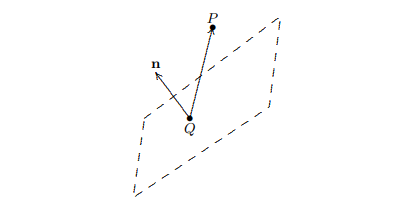
\includegraphics[scale=0.6]{12_5_plane_dist.png}
%		
%		\item The distance from a point $P$ to a line is the shortest distance 
%from $P$ to any point on the line.  Use this and a well-chosen cross product 
%to 
%compute the distance from the point $P=(-1,2,1)$ to the line $\langle 
%1,1,1\rangle+t\langle 2,3,-1\rangle$.\\
%		
%		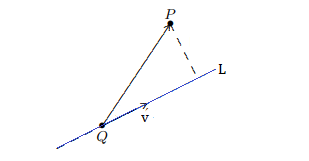
\includegraphics[scale=0.7]{12_5_line_dist.png}
%	\end{enumerate}

\end{enumerate}
}{}

\iftoggle{answers}{
\begin{center}{\large \textbf{Math 2551 Worksheet Answers: Lines and Planes}}
\end{center}


\begin{enumerate}
	
	\item 
	\begin{enumerate}
		\item $\br(t)=\langle 1 -2t, 2-2t, -1+2t\rangle$
		
		\item $\br(t)=\langle t, -7+2t,2t\rangle$
		
		\item $\br(t)=\langle 1+14t, 2t, 15t\rangle$
	\end{enumerate}
	
	\item vector: $3\bi-3\bj+3\bk$.
	
	plane: $3(x-2)-3(y-1)+3(z+1)=0$
	
	\item many correct solutions; pick two distinct points off of the line $PQ$ which are not collinear with the given points.  Two such planes are $-2(x-1)+3(y+1)+5(z-1)=0$ and $-3(x-1)+3(y+1)+3(z-1)=0$.
	
	\item $(2,7,3)$
	
	\item  Parallel: $\langle A_1, B_1, C_1\rangle = \lambda \langle A_2, B_2, C_2\rangle$ for some $\lambda\neq 0$
	
	Perpendicular:  $\langle A_1, B_1, C_1\rangle \dotp \langle A_2, B_2, C_2\rangle=0$
	
	\item $(4,1,3)$
%	\item \begin{enumerate}
%		\item distance $= \dfrac{\vec{QP}\cdot\bn}{\bn}$ with $Q=(1,0,1)$ (any 
%point on the plane works).  So the distance is $\dfrac{\langle 
%0,2,2\rangle\cdot\langle2,-1,3\rangle}{|\langle 
%2,-1,3\rangle|}=\dfrac{4}{\sqrt{14}}$
%		
%		\item distance is $|\vec{QP}|\sin(\theta)=\dfrac{|\vec{QP}\times 
%\bv|}{|\bv|}$ where $Q=(1,1,1), \bv=\langle 2,3,-1\rangle$ (any point on the 
%line and any direction vector works). So the distance is 
%$\dfrac{\sqrt{69}}{\sqrt{14}}$.
%	\end{enumerate}
\end{enumerate}
}{}
\iftoggle{solutions}
{
Solutions go here in the same format.
}{}

% 
\fancyhead[C]{Section 12.6}
\fancyhead[R]{\dayfour}

\iftoggle{questions}{
\begin{center}{\large \textbf{Math 2551 Worksheet: Quadric Surfaces}}
\end{center}


\begin{enumerate}
	
	\item For the following, identify and describe (for example, which way is it oriented? what are the cross-sections?) the type of surface.
	
	\begin{enumerate}
		\item $x^2+4z^2=16$.
		
		\item $9x^2+z^2+y^2=9$.
		
		\item $y^2=3x^2+3z^2$.
		
		\item $z=x^2+y^2+4$.
		
		\item $x^2+y^2=16-z^2$
		
	\end{enumerate}
\end{enumerate}
}{}

\iftoggle{answers}{
\fancyhead[R]{\dayfour}
\begin{center}{\large \textbf{Math 2551 Worksheet Answers: Quadric Surfaces}}
\end{center}


\begin{enumerate}
	\item 	
	\begin{enumerate}
		\item elliptical cylinder, oriented along the $y$-axis, cross-sections are ellipses in the $y=k$ planes or vertical/horizontal lines in the $x=k$ and $z=k$ planes.
		
		\item ellipsoid, centered at the origin, wider in the $z$ and $y$ directions than the $x$ direction, cross-sections are circles in the $x=k$ planes (if $k<1$), ellipses in the $z=k$ and $y=k$ planes ($k<3$)
		
		\item circular cone, oriented along the $y$-axis, cross sections are circles in the $y=k$ planes and lines in the $x=k$ and $z=k$ planes
		
		\item elliptical paraboloid, oriented in the positive $z$ direction, shifted up $4$ units, cross-sections are circles in the $z=k$ planes for $k\geq 4$ and parabolas in the $x=k$ or $y=k$ planes
		
		\item sphere, centered at $(0,0,0)$, radius $4$, cross-sections are circles in $x=k, y=k,$ and $z=k$ planes for $0\leq k\leq 4$.
		
	\end{enumerate}
\end{enumerate}
}{}
\iftoggle{solutions}
{
Solutions go here in the same format.
}{}

% 
\fancyhead[C]{Section 13.1}
\fancyhead[R]{\dayfour}

\iftoggle{questions}{
\begin{center}{\large \textbf{Math 2551 Worksheet: Curves in Space and Their Tangents}}
\end{center}


\begin{enumerate}

	\item Describe the graph of the curve $\br(t)=\langle t\cos(t), t\sin(t), t\rangle$, $t\in\R$.\\
	
	\item Find a vector-valued function for the curve of intersection of the cylinder $x^2+y^2=9$ and the plane $y+z=2$.
	
	\textit{Hint: How could you parameterize the circle $x^2+y^2=9$ in the plane?}\\
	
	\item What is the difference between the parameteric curves $\bff(t)=\langle t, t,t^2\rangle, \bg(t)=\langle t^2, t^2, t^4\rangle$, and $\bh(t)=\langle \sin(t),\sin(t),\sin^2(t)\rangle$ as $t$ runs over all real numbers?\\
	
	\item With a parametric plot and a set of $t$ values, we can associate a `direction'.  For example, the curve $\langle \cos(t),\sin(t)\rangle$, $t\in[0,2\pi]$ is the unit circle traced counterclockwise.  How can we change a set of given parametric equations and $t$ values to get the same curve, only traced backwards?
	
	\item The motion of a particle in the $xy$-plane at time $t$ is described by the vector function
	\[\br(t)= e^{t}\bi + \frac{2}{9}e^{2t}\bj\]
	\begin{enumerate}
		\item Find an equation in $x$ and $y$ whose graph is the path of the particle. Consider how $y(t)$ is related to $x(t)$ and what values $x(t)$ takes on.
		
		\item Find the particle's velocity and acceleration vectors at $t=\ln(3).$
		
		\item Sketch the path of the particle and include the particle's velocity and acceleration vectors at $t=\ln(3).$
	\end{enumerate}
	
	\item Find the parametric equations for the line that is tangent to the curve \\
	\[\vect r(t)=\left\langle \ln t, \frac{t-1}{t+2}, t \ln t \right\rangle, \text{ at } t = 1.\]
	
	\item Determine the point at which $\bff(t)=\langle t, t^2,t^3\rangle$ and $\bg(t)=\langle \cos(t), \cos(2t), t+1\rangle$ intersect, and find the angle between the curves at that point. (Hint: You'll need to set this up like the line intersection problems you've seen before, writing one in $s$ and one in $t$). 
	
	If these two functions were the trajectories of two bumblebees on the same scale of time, would the bees collide at their point of intersection? Explain.
	
	\item Find the equation of the plane perpendicular to the curve $\langle \cos(t),\sin(t),\cos(6t)\rangle$ when $t=\pi/4$.
\end{enumerate}
}{}

\iftoggle{answers}{
\fancyhead[R]{\dayfour}
\begin{center}{\large \textbf{Math 2551 Worksheet Answers: Curves in Space and Their Tangents}}
\end{center}


\begin{enumerate}

	\item This curve's graph is a spiral, narrowing to a point at the origin when $t=0$ and widening outward around the $z$-axis for larger/smaller $t$.\\
	
	\item $\br(t)=\langle 3\cos(t), 3\sin(t),2-3\sin(t)\rangle, 0\leq t\leq 2\pi$.\\
	
	\item  All three functions describe part of the same set of points in $\R^3$, which lie above the line $y=x$ in the $xy$-plane and form a parabola in the plane $x=y$.  $\bff$ traces out all of the points on this parabola, $\bg$ only those in the first octant, and $\bh$ only those which lie above the square $[-1,1]\times[-1,1]$.\\
	
	\item Many possible answers; depending on the domain and functions involved.  If the domain is bounded, e.g. $[a,b]$, then letting $s=b+(a-b)t$ and taking $\br(s)$ as the new parametric equations works. If the domain is $(-\infty,\infty)$, we can just let $s=-t$.
	
	
	\item 
	\begin{enumerate}
		\item $y=\dfrac{2}{9}x^2$ for $x>0$
		
		\item $\bv(\ln(3))=3\bi+4\bj$
		
		$\ba(\ln(3))=3\bi+8\bj$.
	\end{enumerate}
	
	\item $x(s)=s, y(s)=\dfrac{s}{3}, z(s)=s$
	
	
	
	\item $(1,1,1)$ (where the first parameter is 1 and the second is 0).  The angle is $\arccos(3/\sqrt{14})$.  The bees would not collide, since the first bee reaches the point at $t=1$ and the second bee at $t=0$.
	
	\item $-\dfrac{1}{\sqrt{2}}(x-\dfrac{1}{\sqrt{2}})+\dfrac{1}{\sqrt{2}}(y-\dfrac{1}{\sqrt{2}})+6(z-0)=0$
	
	OR $x-y-6\sqrt{2}z=0$
\end{enumerate}
}{}
\iftoggle{solutions}
{
Solutions go here in the same format.
}{}

% 
\fancyhead[C]{Section 13.2}
\fancyhead[R]{\dayfive}

\iftoggle{questions}{\begin{center}{\large \textbf{Math 2551 Worksheet: Integrals of Vector Valued Functions}}
\end{center}

\begin{enumerate}
	
	
	
	
	\item Suppose that $\br(t)$ satisfies 
	\[
	\br''(t)=-\bi-\bj-\bk, \quad t\geq 0, \qquad \br'(0)=5 \bi, \qquad \br(0)=10\bi+10\bj+10\bk
	\]
	Find $\br(t)$.
	
	\item A baseball is hit when it is $2.5$ ft above the ground. It leaves the bat with an initial velocity of $140$ ft/sec at a launch angle of $30^\circ$. At the instant the ball is hit, an instantaneous gust of wind blows against the ball, adding a component of $-14 \hat{i}$ (ft/sec) to the ball's initial velocity. A $15$ ft high fence lies $400$ ft from the home plate in the direction of the flight. (Note that gravity, g $= 32$ ft/sec$^2$)
	
	\begin{enumerate}
		\item Include an appropriate sketch.
		
		\item Find a vector equation for the path of the baseball.
		
		\item How high does the baseball go, and when does it reach maximum height?
		
		\item Find the range and flight time of the baseball, assuming that the ball is not caught.
		
		\item When is the baseball $20$ ft high? How far (ground distance) is the baseball from home plate at that height?
		
		\item Has the batter hit a home run? Explain.
	\end{enumerate}	
	
\end{enumerate}
}{}

\iftoggle{answers}{
\fancyhead[R]{\dayfive}
\begin{center}{\large \textbf{Math 2551 Worksheet 5 Answers: Calculus of Vector-Valued Functions}}
\end{center}

\begin{enumerate}
	
	\item $\br(t)=\langle -\dfrac{1}{2}t^2+5t+10,-\dfrac{1}{2}t^2+10,-\dfrac{1}{2}t^2+10\rangle, \quad t\geq 0$.
	\item A baseball is hit when it is $2.5$ ft above the ground. It leaves the bat with an initial velocity of $140$ ft/sec at a launch angle of $30^\circ$. At the instant the ball is hit, an instantaneous gust of wind blows against the ball, adding a component of $-14 \hat{i}$ (ft/sec) to the ball's initial velocity. A $15$ ft high fence lies $400$ ft from the home plate in the direction of the flight. (Note that gravity, g $= 32$ ft/sec$^2$)
	
	\begin{enumerate}
		\item Sorry, no sketch. :)
		
		\item $\vect r(t) = (140\cos 30^\circ-14)t \hat{i}+ (2.5+(140\sin 30^\circ)t-16t^2)\hat{j} = (70\sqrt{3} -  14) t \hat{i} + (2.5+70t-16t^2) \hat{j}$.
		
		\item $y_{\text{max}}=\frac{(140 \sin 30^\circ)^2}{64}+2.5=\frac{70^{2}}{64}+2.5 = 79.0625$ ft., which is reached at $t = \frac{140 \sin 30^\circ}{32}=\frac{70}{32}=2.1875$ s.
		
		\item For the time, solve $y=2.5+70t-16t^2=0$ for $t$. Using quadratic formula, we have $t=4.41$s. Then, the range at $t=4.41$ is $x(4.41) = (140\cos 30^\circ-14)(4.41)=472.94$ ft. 
		
		\item For the time, solve $y=2.5+70t-16t^2=20$ for $t$. Using quadratic formula, we have $t=0.27, \ 4.11$ seconds. Then, the range at those times are $x(0.27) = 29$ ft and $x(4.11)=441$ ft.
		
		\item Yes, according to part (d), the ball is still 20 feet above the ground when it is 441 feet from home plate.
	\end{enumerate}	

\end{enumerate}
}{}
\iftoggle{solutions}
{
Solutions go here in the same format.
}{}

% 
\fancyhead[C]{Section 13.3}
\fancyhead[R]{\dayfive}

\iftoggle{questions}{\begin{center}{\large \textbf{Math 2551 Worksheet: Arc Length}}
\end{center}

\begin{enumerate}	

	\item Let $\br(t)=\langle 6 \sin 2t, 6 \cos 2t, 5t\rangle $. Find the unit tangent vector of $\br(t)$ and find the length of the portion of the graph of $\br(t)$ where $0 \leq t \leq \pi$.
	
	
	\item Find the point on the curve
	\[
	\br(t) = (5 \sin t)\bi+(5 \cos t)\bj+12t\bk
	\]
	at a distance $26\pi$ units along the curve from the point $(0,5,0)$ in the direction of increasing arc length.
	
	\item Suppose an object's position is given by $\br(t)= (2\ln (t+1))\bi+(e^{2t}+t)\bj+(\sin^2(t))\bk$. Set up but do not evaluate the appropriate integral with limits to find the distance the object traveled from the point $A(0,1,0)$ to the point $B(\ln 4,e^2+1,\sin^2(1))$.
	
	\item Find the length of the curve 
	\[
	\br(t) = \langle\sqrt{2}t,\sqrt{3}t,(1-t)\rangle
	\]
	from $(0,0,1)$ to $(\sqrt{2}, \sqrt{3}, 0)$.
\end{enumerate}
}{}

\iftoggle{answers}{\begin{center}{\large \textbf{Math 2551 Worksheet Answers: Arc Length}}
\end{center}

\begin{enumerate}	


\item $\bT(t)=\dfrac{1}{13}\langle 12\cos(2t),-12\sin(2t),5\rangle $

length: $13\pi$


\item $(0,5,24\pi)$

\item $\Ds \int_0^1 \sqrt{(\dfrac{2}{t+1})^2+(2e^{2t}+1)^2+(2\sin(t)\cos(t))^2}\ dt$

\item $\sqrt{6}$

\end{enumerate}
}{}
\iftoggle{solutions}
{
Solutions go here in the same format.
}{}

% 
\fancyhead[C]{Section 13.4}
\fancyhead[R]{\daysix}

\section*{\centering Chapter 13.4: Curvature and Normals}

\textbf{G3: Geometry of Curves.} I can compute the arc length of a curve in two or three dimensions and apply arc length to solve problems. I can compute normal vectors and curvature for curves in two and three dimensions.  I can interpret these objects geometrically and in applications.

\vspace{-.5cm}

\subsection*{Mechanics}
\begin{enumerate}	
	
	\item \question{Find $\bT, \bN$ and $\kappa$ for the curve $\br(t)=\cos(2t)\bi-\sin(2t)\bj+6t\bk$, for $t \geq  0$. What do you notice about $\kappa$? Explain (perhaps with a picture) why this happens. }
    { %answer
    $\bT(t)=\dfrac{1}{\sqrt{10}}(-\sin(2t)\bi-\cos(2t)\bj+3\bk)$, 
    
    $\bN(t)=-\cos(2t)\bi+\sin(2t)\bj$

    $\kappa(t)=\dfrac{1}{10}$. The curvature is constant.
    }
    { %solution
    }

	\item \question{Compute the unit tangent vector, unit normal vector, and curvature of the curve $\br(t)=\langle \sqrt{2} t, 1+t, e^t\rangle$ for all $t\in\R$.}
    { %answer
    $\bT(t) = \dfrac{1}{\sqrt{3 + e^{2t}}}\langle \sqrt{2}, 1, e^t\rangle,$ 

    $\bN(t) = \dfrac{1}{\sqrt{9+3e^{2t}}} \langle -\sqrt{2}e^{t}, -e^{t}, 3 \rangle,$ 

    $\kappa(t) = \dfrac{\sqrt{3}e^t}{(3 + e^{2t})^{3/2}}.$
    }
    { %solution
    }
	
    \item \question{Compute $\bN$ for the curve $\br(t)=\langle t, (1/3)t^3\rangle, t\in\R$ for $t\neq 0$.
    
	Does $\bN$ exist at $t=0$? Graph the curve, along with its normal vectors at the times $t=-1,-0.5,0.5,1$ and explain what is happening to $\bN$ as $t$ passes through $(0,0)$}
    { %answer
        $\bN=\langle \dfrac{-t^2}{\sqrt{1+t^4}}, \dfrac{1}{\sqrt{1+t^4}}\rangle$ if $t>0$ and $\langle \dfrac{t^2}{\sqrt{1+t^4}}, \dfrac{-1}{\sqrt{1+t^4}}\rangle$ if $t<0$.

        The normal vector does not exist when $t=0$; as $t$ passes from negative to positive values the normal vector changes which side of the curve it is on.
    }
    { %solution
    }
\end{enumerate}

\vspace{-.5cm}
\subsection*{Applications}
\begin{enumerate}[resume]
	\item \question{You are an engineer overseeing the construction of a certain bridge on campus. The blueprint shows that the bridge has a side view profile which looks like the parabola $y=x^2$. Unfortunately, the material that the bridge is supposed to be built with is extremely rigid, and can only support curves with $\kappa \leq 1.5$ units. Can this bridge be safely built with this material? [\textit{Hint: Where is the curvature the greatest?}]}
    {It cannot; the greatest curvature is \(\kappa =2\) units.}
    {The point of greatest curvature occurs at $x=0$. Using the 
parameterization $\br(t)=\langle t, t^2\rangle$ gives 
$\kappa(t)=\dfrac{2}{(1+4t^2)^{3/2}}$, which is maximized when $t=0$.}
	
    \item \question{Imagine that you are an ant travelling along the space curve \begin{equation*}
        \br_1(t) = \left(\frac{3}{2}t^2+2t,4t-1,-3t^2+10t\right)
    \end{equation*} 
    while your ant-friend is travelling along a different space curve \begin{equation*}
        \br_2(t) = \left(2t^2-3t+10,-\frac{1}{2}t^2+9t,-2t^2\right)
    \end{equation*}
    Assuming you are both looking ``forwards'' and are on the same scale of time, is there a time $t$ when you are both looking in the same direction? If so, at what time? }
    { %answer
        Yes, at $t=5$.
    }
    { %solution
    }
\end{enumerate}

\vspace{-.5cm}
\subsection*{Extensions}
\begin{enumerate}[resume]
    \item \question{For a smooth curve $\br(t)$, define its \textit{binormal vector} $\mathbf{B}(t)$ at a time $t$ to be $\mathbf{B}(t)=\bT(t)\times \bN(t)$, where the $\times$ is the vector cross product. Compute $\mathbf{B}$ for $\br(t) = (t,3\cos t, 3\sin t)$. }
    { %answer
        $\mathbf{B}(t)=\dfrac{1}{\sqrt{10}} \langle 3, \sin(t), -\cos(t)\rangle$
    }
    { %solution
    }
    
	\item \question{Give an example of a parametric curve in $\mathbb{R}^2$ which has $ \bN (t) = \left(\frac{-3}{\sqrt{e^{2t}+9}},\frac{e^t}{\sqrt{e^{2t}+9}}\right)$. You may want to use the fact that $\|(e^t,3)\| =\sqrt{e^{2t}+9}$. [\textit{Hint: First deduce a possible $\bT$, then use the given fact, and integrate.}]}
	{ %answer
        $\br(t) = \langle -e^t, -3t\rangle$
    }
    { %solution
    }
\end{enumerate}
% 
\fancyhead[C]{Section 14.1}
\fancyhead[R]{\dayseven}

\iftoggle{questions}{
\begin{center}
	{\large \textbf{Math 2551 Worksheet: Multivariable Functions}}
\end{center}

\begin{enumerate}	
	\item Find and sketch the domain for each function.
	\begin{enumerate}
		\item $f(x,y)=\sqrt{x-y-1}.$
		
		\item $f(x,y) = \sqrt{(x-4)(y^2-1)}.$
		
		\item $f(x,y)=\cos^{-1}(y-4x^2)$.
		
		\item $f(x,y)= \dfrac{1}{4-x^2-y^2}.$
		
		\item $f(x,y)=\dfrac{1}{\ln(4-x^2-y^2)}$
	\end{enumerate}
	
	\item Match the surfaces (a)-(g) with the written descriptions of the level curves (A)-(F).  You may use each description once, multiple times, or not at all.
	
	\begin{minipage}[c]{0.3\linewidth}
		\begin{enumerate}
			\item $z=2x^2+3y^2$
			\item $z=x^2+y^2$
			\item $z=\dfrac{1}{x-1}$
			\item $z=2x+3y$
			\item $z=\sqrt{25-x^2-y^2}$
			\item $z=\sqrt{x^2+y^2}$
			\item $z=xy$.
		\end{enumerate}
	\end{minipage} % no space if you would like to put them side by side
	\begin{minipage}[c]{0.7\linewidth}
		\begin{enumerate}[label=(\Alph*)]
			\item a collection of unequally spaced concentric circles
			\item a collection of unequally spaced parallel lines
			\item a collection of equally spaced concentric circles
			\item two straight lines and a collection of hyperbolas
			\item a collection of concentric ellipses
			\item a collection of equally spaced parallel lines
		\end{enumerate}
	\end{minipage}
	
	\item Find an equation for the level curve of the function $F(x,y)=\dfrac{2y-x}{x+y+1}$ passing through $(-1,1)$.
	
	\item Find the equation for the level surface of the function $f(x,y,z)=\sqrt{x^2+y^2+z^2}$ passing through $(1,1,1)$. 
	
	\item Let $f(x,y) = (x-y)^2$. Determine the equations and shapes of the cross-sections when $x = 0$, $y = 0$, and $x = y,$ and describe the level curves. Use this information to produce a sketch of the graph of the surface.  Confirm your sketch using a 3d graphing utility.
\end{enumerate}
}{}

\iftoggle{answers}{
\begin{center}
	{\large \textbf{Math 2551 Worksheet Answers: Multivariable Functions}}
\end{center}

\begin{enumerate}	
	\item Find and sketch the domain for each function.
	\begin{enumerate}
		\item $\{ (x,y)\mid x-y\geq 1 \}$
		
		\item $\{ (x,y) \mid x\geq 4, |y|\geq 1 \} \cup \{(x,y) \mid x<4, |y|<1 \}$
		
		\item $\{ (x,y) \mid 4x^2-1\leq y\leq 4x^2+1 \}$
		
		\item All of $\R^2$ except the circle $x^2+y^2=4$
		
		\item All of the disk $x^2+y^2< 4$ except the circle $x^2+y^2=3$.
	\end{enumerate}
	
	\item	
	\begin{enumerate}
		\item  a collection of concentric ellipses
		\item a collection of unequally spaced concentric circles
		\item a collection of unequally spaced parallel lines
		\item a collection of equally spaced parallel lines
		\item a collection of unequally spaced concentric circles
		\item a collection of equally spaced concentric circles
		\item two straight lines and a collection of hyperbolas
	\end{enumerate}
	
	\item The plane $4x+y+3=0$, except for those points with $x+y=-1$.
	
	\item The sphere $3=x^2+y^2+z^2$
	
	\item When $x=0$, the cross-section is the parabola $z=y^2$. 
	
	When $y=0$, the cross-section is the parabola $z=x^2$.
	
	When $x=y$, the cross-section is the line $z=0$.
	
	The level curves are pairs of parallel lines $y=x\pm\sqrt{k}$.
\end{enumerate}
}{}
\iftoggle{solutions}
{
Solutions go here in the same format.
}{}

% 
\fancyhead[C]{Section 14.2}
	\fancyhead[R]{\dayseven}
\iftoggle{questions}{	
\begin{center}{\large \textbf{Math 2551 Worksheet: Limits and Continuity}}
\end{center}


\begin{enumerate}	
	\item  Let $f(x,y)=\left(\dfrac{1}{x}+\dfrac{1}{y}\right)^2$. Find $\displaystyle \lim_{(x,y) \to (2,-3)} f(x,y)$ or show it does not exist.
	
	\item Let $f(x,y)= \dfrac{x-2y}{x^3-8y^3}$.  Find $\displaystyle \lim_{(x,y) \to (2,1)} f(x,y)$ or show it does not exist.
	
	\item Let $f(x,y) = \dfrac{\sqrt{2x-y}-2}{2x-y-4}$.  Find $\displaystyle \lim_{(x,y) \to (2,0)} f(x,y)$ or show it does not exist.
	
	\item Let $f(x,y)= \dfrac{y^2}{x^2+y^2}$.  Find $\displaystyle \lim_{(x,y) \to (0,0)} f(x,y)$ or show it does not exist.
	
	\item At what points $(x,y)$ in the plane is $f(x,y)=\cos\left(\dfrac{1}{xy}\right)$ continuous?  
	\item At what points $(x,y,z)$ is $h(x,y,z)= \dfrac{1}{1-\ln{(x^2+y^2+z^2)}}$ continuous?
	
\end{enumerate}
}{}

\iftoggle{answers}{
\begin{center}{\large \textbf{Math 2551 Worksheet Answers: Limits and Continuity}}
	\end{center}
\begin{enumerate}	
	\item  $\dfrac{1}{36}$
	
	\item $\dfrac{1}{12}$
	
	\item $\dfrac{1}{4}$
	
	\item Does not exist.
	
	\item $f$ is continuous on its entire domain: all $(x,y)$ such that neither $x=0$ nor $y=0$.
	
	\item $f$ is continuous on its entire domain: all $(x,y,z)$ except the sphere $x^2+y^2+z^2=e$.
\end{enumerate}
}{}
\iftoggle{solutions}
{
Solutions go here in the same format.
}{}
% 
\fancyhead[C]{Sections 12.1-6, 13.1-4, 14.1-2}
\fancyhead[R]{\dayeight}
	
\iftoggle{questions}{\begin{center}{\large \textbf{Math 2551 Worksheet 8 - Review for Exam 1}}
\end{center}


\begin{enumerate}	
	\item Set up the integral to find the arc length of the curve $y=e^x$ from the point $(0,1)$ to the point $(1,e)$.  Focus on finding a parameterization, and on what values of $t$ give these two points.  Is this an integral you would want to compute? Why or why not?
	
	\item Parameterize the line tangent to the curve 
	\[ \br(t)=\langle \cos^2(t),\sin(t)\cos(t),\cos(t)\rangle \]
	at the point where $t=\pi/2$.
	
	\item Compute the unit tangent vector $\bT(t)$ and the unit normal vector $\bN(t)$ to the circle 
	\[\br(t)=\langle 2\cos(t),2\sin(t)\rangle. \]
	Before checking, should the normal vector be pointing into or out of the circle? Why?
	
	\item We have seen that the curvature of a circle with radius $a$ is $1/a$.  Thinking about the geometry of a helix with radius $a$, do you think its curvature will be greater than or less than $1/a$?  Why?  Compute the curvature using the parameterization 
	\[\br(t)=\langle a\cos(t), t, a\sin(t) \rangle \]
	to confirm or challenge your intuition.
	
	\item The function $\mathbf{\ell}(t)$ below describes a line.  There is a particular plane that $\mathbf{\ell}(t)$ is normal to at the point $t=0$.  Find an equation of this plane.
	\[\mathbf{\ell}(t)=\langle 3-3t,2+t,-2t\rangle. \]
	
	Where does this line intersect the different plane $3x-y+2z=-7$?
	
	\item Find and sketch the domain of each of the following functions of two variables:
	\begin{enumerate}
		\item $\sqrt{9-x^2}+\sqrt{y^2-4}$
		\item $\arcsin(x^2+y^2-2)$
		\item $\sqrt{16-x^2-4y^2}$
	\end{enumerate}

	\item Solve the differential equation below, together with its given initial conditions.  Remember that this means finding all functions $\br(t)$ which satisfy the given equations.
	
		\[ \br''(t)=2\bi+6t\bj+\dfrac{1}{2\sqrt{t}}\bk, \quad \br'(1)=2\bi+3\bj+\bk, \quad \br(1)=\bi+\bj \]
		
		
		
		\item Let $f(x,y)=(x^2-y^2)/(x^2+y^2)$ for $(x,y)\neq (0,0)$. Is it possible to define $f(0,0)$ in a way that makes $f$ continuous at the origin? Why?
	
\end{enumerate}
}
\iftoggle{answers}{

\begin{center}{\large \textbf{Math 2551 Worksheet 8 Answers - Review for Exam 1}}
\end{center}


\begin{enumerate}	
	\item $\int_0^1 \sqrt{1+e^{2t}}\ dt$
	
	\item $\mathbf{\ell}(s)=\langle 0,-s,-s\rangle$
	
	\item $\bT(t)=\langle -\sin(t),\cos(t)\rangle$
	
	$\bN(t)=\langle -\cos(t),-\sin(t)\rangle$
	
	Into
	
	\item $\kappa=\dfrac{a}{1+a^2}$
	
	\item $-3(x-3)+(y-2)-2z=0$ \\
	Intersection point is $(0,3,-2)$, when $t=1$.
	
	\item \begin{enumerate}
		\item $\{(x,y)\mid |x|\leq 3,|y|\geq 2 \}$
		\item $1\leq x^2+y^2\leq 3$
		\item $\dfrac{x^2}{16}+\dfrac{y^2}{4}\leq 1$
	\end{enumerate}

	\item $\br(t)=t^2\bi+t^3\bj+\frac{2}{3}(t^{3/2}-1)\bk$
	\item No, because the limit of $f$ as $(x,y)\to(0,0)$ does not exist.
\end{enumerate}
}{}
\iftoggle{solutions}
{
Solutions go here in the same format.
}{}

% 
\fancyhead[C]{Section 14.3}
\fancyhead[R]{\daynine}
\iftoggle{questions}
{\begin{center}{\large \section*{\centering Chapter 14.3: Partial Derivatives}}
\end{center}
\subsection*{Mechanics}
\begin{enumerate}
    \item Find all first and second partial derivatives for $f(x,y)=e^x+x\ln (y).$
    \item Find $f_x$, $f_y$, $f_z$, and $f_{xzz}$ for the function $f(x,y,z)=x\sin(yz)$.
 \item Find the total derivative $Df$ at the given point for each function below. Remember that $Df$ is the matrix of (partial) derivatives of the function and if $f$ is a function from $\R^n$ to $\R^m$ then $Df$ is a $m\times n$ matrix.
	\begin{enumerate}
		\item $f(x)=2x^3+7$ at $x=2$.
		\item $\mathbf{f}(t)=\langle 2\cos(t), 2 \sin(t), t\rangle$ at $t=\pi/2$.
		\item $f(x,y)=\sqrt{y-x}$ at $(x,y)=(1,2)$.
		\item $f(x,y,z)=e^{2y-x}+z^2+4$ at $(x,y,z)=(1,2,3)$.
		\item $\mathbf{f}(s,t) = \langle 2s+3t, t-s\rangle$ at $(s,t)=(1,1)$.  
	
		\textbf{Note:} The graph of this function is a surface (in this case all of $\R^2$) parameterized by two variables just like the graph of the function in (b) is a curve parameterized by one variable - we'll see these more later!  Another way of thinking about this is that this is a \textit{change of variables} for $\R^2$ between the system of coordinates $(s,t)$ and $(x,y)$.
	\end{enumerate}
    
\end{enumerate}
\subsection*{Applications}
\begin{enumerate}[resume]
    \item The speed of sound $C$ traveling through ocean water is a function of 
	temperature, salinity, and depth.  It may be modeled by the function	
	\[C(T,S,D)=1450 +4.5T-0.05T^2+0.0003T^3+(1.5-0.01T)(S-35)+0.015D, \]
	
	where $C$ is the speed of sound in meters/second, $T$ is the temprature in degrees Celsius, $S$ is the salinity in grams/liter of water, and $D$ is the depth below the ocean surface in meters.
	
	\begin{enumerate}
		\item State the units in which each of the partial derivatives $C_T,C_S,$ and $C_D$ are expressed and explain the physical meaning of each.
		
		\item Find the partial derivatives $C_T, C_S,$ and $C_D$.
		
		\item Evaluate each of the three partial derivatives at the point where $T=10, S=35$, and $D=100$.  What does the sign of each partial derivative tell us about the behavior of the function $C$ at the point $(10,35,100)$?
	\end{enumerate}
    \pagebreak 
    
    \item Recall from last week's worksheet that a utility function is a multivariable function $u(x,y,z)$, where $x,y,z$ represent three independent properties of an object (eg., price, quantity, quality), and $u$ tells you how much you value that item. The \textit{marginal utility functions} are the partial derivatives $u_x,u_y$ and $u_z$. What is the economic interpretation of the marginal utilities? 
\end{enumerate}
\subsection*{Extensions}
\begin{enumerate}[resume]
	
	\item Below is a contour plot for a function $f(x,y)$, with values for some of the contours (level curves) indicated on the \textit{left} of the figure.
	
	\begin{minipage}{0.6\textwidth}
		\begin{enumerate}
			\item Find the sign of the partial derivatives \\
            $f_x(-2,-1)$ and $f_y(-2,-1)$.
			\item At the point $(0,-1/2)$, which is larger? $f_x$ or $f_y$?
			\item Find all $(x,y)$ where $f_x(x,y)=0$.
			\item Locate, if possible, one point $(x,y)$ where\\ $f_x(x,y)<0$.
		\end{enumerate}
	\end{minipage}
	\begin{minipage}{0.4\textwidth}
		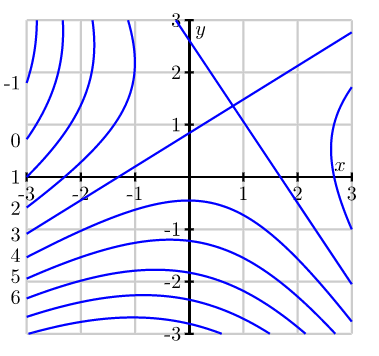
\includegraphics[scale=0.6]{contour_14_3.png}
	\end{minipage}
	

	

%	\item Find $f_x$ and $f_y$ for:
%	\begin{enumerate}
%		\item $f(x,y)= x^3y^2+5y^2-x+7$
%		
%		\item $f(x,y) = e^{x^2y^3} \sqrt{x^2+1}$
%		
%		\item $f(x,y) = \cos(xy^2)+\sin(x)$
%	\end{enumerate}

	\item The fifth-order partial derivative $\partial^5f/\partial x^2\partial y^3$ is zero for each of the following functions.  To show this as quickly as possible, which variable would you differentiate with respect to first: $x$ or $y$?
	
	Try to answer without writing anything down.  Why did you make the choice you did?
	
	\begin{enumerate}
		\item $f(x,y)=y^2x^4e^x+2$
		
		\item $f(x,y)=y^2+y(\sin(x)-x^4)$
		
		\item $f(x,y)=x^2+5xy+\sin(x)+7e^x$
		
		\item $f(x,y)=xe^{y^/2}$
	\end{enumerate}
    \item Let $A$ be any $2\times 2$ matrix, and let $\mathbf{f}: \mathbb{R}^2\to\mathbb{R}^2$ be given by $\mathbf{f}(\mathbf{x}) = A\mathbf{x}$. Compute the total derivative $D\mathbf{f}$. What do you notice? What familiar family of functions from Calc 1 does this remind you of? Can you generalize this result? 
\end{enumerate}
}{}

\iftoggle{answers}{
\begin{center}{\large \textbf{Math 2551 Worksheet Answers: Partial Derivatives}}
\end{center}
\begin{enumerate}	
	\item 
	\begin{enumerate}
		\item $f_x(-2,-1)\approx 0.75$
		\item $f_y(-2,-1)\approx 1.5$
		\item There are several possible points (these are places where the tangent to a contour is horizontal): $(0,-.5),(-.5,-1.25)$, etc.
		\item Again, there are many possible points; any point on the 4, 5, 6 contours in quadrant IV will work.
	\end{enumerate}

	\item \begin{enumerate}
		\item $C_T$: (meters/second)/ degree Celsius - this gives the change in speed for each one degree C of temperature increase.
		$C_S$ (meters/second)/(grams/liter) - this gives the change in speed for each one gram/liter increase in salinity
		$C_D$: (meters/second)/meter - this gives the change in speed for each one meter increase in depth below the surface
		
		\item $C_T= 4.5-0.1T+0.0009T^2-0.01(S-35)$
		$C_S=1.5-0.01T$
		$C_D=0.015$
		
		\item At $(T,S,D)=(10,35,100)$, we have $C_T=3.59, C_S=1.4, C_D=0.015$.  This tells us that if we increase the temperature, salinity, or depth from these conditions the speed of sound will increase as well.
	\end{enumerate}
%	\item 	\begin{enumerate}
%		\item $f_x=3x^2y^2-1, f_y=2x^3y+10y$
%		
%		\item $f_x=2xy^3e^{x^2y^3}\sqrt{x^2+1}+\dfrac{x e^{x^2y^3}}{\sqrt{x^2+1}}, f_y=3x^2y^2 e^{x^2y^3}\sqrt{x^2+1}$
%		
%		\item $f_x=-y^2\sin(xy^2)+\cos(x), f_y=-2xy\sin(xy^2)$
%	\end{enumerate}
	
	\item $f_{xx}=e^x, f_{xy}=f_{yx}=\dfrac{1}{y}, f_{yy}=-\dfrac{x}{y^2}$
	
	\item $f_x=\sin(yz), f_y=xz\cos(yz), f_z=xy\cos(yz), f_{xzz}=-y^2\sin(yz)$
	
	\item Find the total derivative $Df$ at the given point for each function below. Remember that $Df$ is the matrix of (partial) derivatives of the function and if $f$ is a function from $\R^n$ to $\R^m$ then $Df$ is a $m\times n$ matrix.
	\begin{enumerate}
		\item $Df(2)=f'(2)=[24]$
		\item $D\mathbf{f}(\pi/2)=\mathbf{f}'(\pi/2)=\begin{bmatrix}
			-2 \\ 0 \\ 1
		\end{bmatrix}$
		\item $Df(1,2)=\begin{bmatrix}
			-1/2 & 1/2
		\end{bmatrix}$
		\item $Df(1,2,3)=\begin{bmatrix}
			-e^3 & 2e^3 & 6
		\end{bmatrix}$
		\item $D\mathbf{f}(1,1) = \begin{bmatrix}
			2 & 3 \\
			-1 &  1
		\end{bmatrix}  $
		
	\end{enumerate}
	\item Note this does not have a definitive right answer - some differences may arise and that's good! Discuss!
	
	\begin{enumerate}
		\item First $y$ since $\partial^3 f/\partial y^3=0$ and the $y$-partial derivatives are easier
		
		\item First $y$, since $\partial^3 f/\partial y^3=0$
		
		\item First $y$, since $\partial^2 f/\partial y^2=0$
		
		\item First $x$, since $\partial^2 f/\partial x^2=0$ and the $x$-partial derivatives are easier.
	\end{enumerate}
	
	A common theme is to work with the variable with lower powers/simpler expressions first when taking mixed partials.
	
\end{enumerate}
}{}
\iftoggle{solutions}
{
Solutions go here in the same format.
}{}

% 
\fancyhead[C]{Section 14.4}
\fancyhead[R]{\dayten}

\section*{\centering Chapter 14.4: The Chain Rule}
\subsection*{Mechanics}
\begin{enumerate}
	\item Use the chain rule to compute the total derivatives of the following at the prescribed points. [\textit{Recall that $Df$ for $f:\mathbb{R}^n\to\mathbb{R}^m$ is an $m\times n$ matrix.}]
    \begin{enumerate}
		\item $f:\mathbb{R}\to\mathbb{R}$ given by $f(t)=h(g(t))$, where $g(t)= (t+1,t^2)$, $h(x,y)=xy$ at $t=2$.
		\item $f:\mathbb{R}^2\to\mathbb{R}$ given by $f(x,y)=(b\circ a)(x,y)$, where $a(x,y)= x\sin y$, $b(t)=8t-t^2$ at $(x,y)=(4,\pi/3)$. 
        \item $f:\mathbb{R}\to\mathbb{R}^2$ given by $f(t)=u(v(t))$, where $v(t)= (1,t,t^2)$, $u(x,y,z) = (xy,yz)$ at $t=1$. 
        \item $f:\mathbb{R}^2\to\mathbb{R}^2$ given by $f(x,y)=h(g(x,y))$, where $g(x,y)=(3x+4y,5x+7y)$, $h(u,v) = (7u-4v,-5u+3v)$ at $(x,y)=(0,0)$. 
	\end{enumerate}
	\item Find the values of $t$ where $\dfrac{dz}{dt}=0$ if $z=3x+4y$, $x=t^2$, and $y=2t$.
	
	\item Let $w(x,y,z)= xy + yz + zx$, where $x= r \cos \theta, \ \ y= r \sin \theta, \ \  z= r \theta.$ 	Find $\dfrac{\partial w}{\partial r}$ and $\dfrac{\partial w}{\partial \theta}$ when $r=2$ and $\theta = \dfrac{\pi}{2}$.

\end{enumerate}
\subsection*{Applications}
\begin{enumerate}[resume]
      \item You are a myrmecologist (ant scientist) studying the behaviour of ants on anthills. You equipped an ant with a tracker to track its motion. Unfortunately, the exact geometry of the hill, as well as the ant's precise motion are too delicate to measure. Fortunately, at time $t=5$ seconds it is known that
	\[ \pdev{z}{x}=5, \quad \pdev{z}{y}=-2, \quad \dfrac{dx}{dt}=3, \quad \dfrac{dy}{dt}=7. \] where $z$ denotes the height of the ant relative to ground height.
	Use this information to determine if the ant is going uphill or downhill (or neither) at $t=5$ seconds. 
    \item The multivariable chain rule is a key tool in modern machine learning. In the big picture, neural networks "learn" parameters through an algorithm called \textit{gradient descent}. This algorithm involves computing total derivatives of long chains of functions in high dimensions, which is in general extremely hard to do. The chain rule tells us that instead of contending with such a long chain of functions all at once, one can instead study each "layer" by itself, then combine everything with matrix multiplication, which is relatively easier. This is called \textit{backpropagation}. 
	
\end{enumerate}
\subsection*{Extensions}
\begin{enumerate}[resume]
    \item Suppose we have a differentiable function $w=g(x,y)$ and $x$ and $y$ are differentiable functions of $t$ and we know the following information.
	\[g(1,0)=1,\ g_x(1,0)=-2,\ g_y(1,0)=2,\ g(-1,2)=3,\ g_x(-1,2)=1,\ g_y(-1,2)=-2,\]
	\[ x(2)=1,\ y(2)=0,\ x(1)=1,\ y(1)=3,\ x'(2)=4,\ y'(2)=-1,\ x'(1)=0,\ y'(1)=2 \]
	
	If possible, find $\dfrac{dw}{dt}(1)$ and $\dfrac{dw}{dt}(2)$ or explain why the given information is not enough to do so.  Which of these pieces of information would you not use at all to compute either value?
    \item Give an example of a nonconstant, differentiable function $f:\mathbb{R}^2\to\mathbb{R}^2$ for which $Df$ is \textbf{not} invertible at $(0,0)$, but invertible at $(1,0)$.
\end{enumerate}
{}

\iftoggle{answers}{
\begin{center}{\large \textbf{Math 2551 Worksheet Answers: Chain Rule}}
\end{center}

\begin{enumerate}
	\item $\dfrac{dz}{dt}(t_0)=1$
	
	\item $t=-4/3$
	
	\item $\dfrac{\partial w}{\partial r}(2,\pi/2)=2\pi$ \qquad $\dfrac{\partial w}{\partial \theta}(2,\pi/2)=-2\pi$
	
	\item $\dfrac{dw}{dt}(2)=-10$.  $\dfrac{dw}{dt}(1)$ cannot be computed from the given information because we do not know the values of $g_x$ or $g_y$ at $(x(1),y(1))=(1,3)$.  We do not use the values of $g(1,0),g(-1,2),g_x(-1,2),g_y(-1,2)$.
\end{enumerate}

}{}
\iftoggle{solutions}
{
Solutions go here in the same format.
}{}

% \fancyhead[C]{Section 14.5}
\fancyhead[R]{\dayeleven}

\section*{\centering Chapter 14.5: Gradients and Directional Derivatives}

\textbf{D1: Computing Derivatives.} I can compute partial derivatives, total derivatives, directional derivatives, and gradients. I can use the Chain Rule for multivariable functions to compute derivatives of composite functions.

\textbf{A1: Interpreting Derivatives.} I can interpret the meaning of a partial derivative, a gradient, or a directional derivative of a function at a given point in a specified direction, including in the context of a graph or a contour plot.

\subsection*{Mechanics}
\begin{enumerate}
    \item \question{Compute the gradients of each of the following: 
    \begin{enumerate}
        \item $f(x,y)=x^2y$
        \item $f(x,y,z)=x\sin (y)+z\cos (x)$
        \item $f(x,y,z,w)=x^2+y^2+z^2+w^2$
    \end{enumerate}}
	{ % answer goes here
        \begin{enumerate}
            \item $\langle 2xy, x^2\rangle$
            \item $\langle \sin(y)-z\sin(x), x\cos(y),\cos(x)\rangle$
            \item $\langle 2x, 2y, 2z,2w\rangle$
        \end{enumerate}
	}
	{ % solution goes here
	}
	
    \item \question{Find the derivative of $g(x,y)= \dfrac{x-y}{xy+2}$ at $(1,-1)$ in the direction of $\langle 12, 5\rangle$}
	{ % answer goes here
		$D_{\bu}g(1,-1)=\dfrac{21}{13}$
	}
	{ % solution goes here
	}

    \item \question{Let $f(x,y)=xy$.  Sketch the curve $f(x,y)= -4$ together with $\nabla f(2,-2)$ and the tangent line at $(2,-2)$. Then, find an equation for the tangent line. What do you notice?}
	{ % answer goes here
	Tangent line: $-2(x-2)+2(y+2)=0$
		
	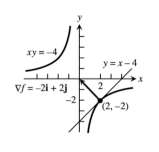
\includegraphics[alt={graph of hyperbola xy=-4 with line -2(x-2)+2(y+2)=0, line tangent to the hyperbola at (2,-2)}]{14_5_sketch_soln.png}
	}
	{ % solution goes here
	}
\end{enumerate}

\subsection*{Applications}
\begin{enumerate}[resume]
    \item \question{Gradients form the basis for "learning" in machine learning through a process called \emph{gradient descent}. Here is a setup and overview of the thematic ideas: we are interested in minimizing a (differentiable) error function $\mathcal{L}(x,y,z)$ (\emph{eg., $\mathcal{L}$ might represent the difference between a predicted quantity vs. the true value}). Though we are able to plug in points, the function $\mathcal{L}$ may be difficult to write down, thus we cannot do "regular calculus" (eg., first derivative test) with it. 
    
    Gradients give us a workaround to approximate a local minimum as follows: start by randomly choosing point $(x_0,y_0,z_0)$. Calculate the gradient at this point, and then take a small step in the direction of $-\nabla \mathcal{L}(x_0,y_0,z_0)$ [why this direction?] to arrive at a new point $(x_1,y_1,z_1)$. Now, repeat this process with successively smaller step sizes. As it turns out, if we choose our initial point and step sizes cleverly, we are (sometimes) able to get closer and closer to a local minimum, without having much knowledge of the function $\mathcal{L}$! Can you anticipate some shortcomings of this algorithm? }
	{ % answer goes here
        Answers will vary.  May include issues with stability or overshooting.
	}
	{ % solution goes here
	}
	
    \item \question{Suppose you are climbing a hill whose shape is given by the equation
	\[ z = 1000 - 0.005x^2-0.01y^2, \]
	where $x, y,$ and $z$ are measured in meters, and you are standing at a point with
	coordinates $(60, 40, 966)$. The positive $x$-axis points east and the positive $y$-axis
	points north.
	\begin{enumerate}
		\item If you walk due south, will you start to ascend or descend? At what rate?
		\item If you walk northwest, will you start to ascend or descend? At what rate?
		\item In which direction is the slope largest? What is the rate of ascent in that direction?
	\end{enumerate} }
	{ % answer goes here
		\begin{enumerate}
			\item Ascend at a rate of 0.8 vertical meters per horizontal meter
			\item Descend at a rate of $\sqrt{2}/10$ vertical meters per horizontal meter
			\item $\langle -0.6, -0.8\rangle$ is the direction of largest slope with rate of ascent 1 vertical meter per horizontal meter.
		\end{enumerate}
	}
	{ % solution goes here
	}
\end{enumerate}

\subsection*{Extensions}
\begin{enumerate}[resume]
	\item \question{Use the contour diagram of the differentiable function f given below to decide if
	the specified directional derivative is positive, negative, or approximately zero.
	
	\begin{minipage}{0.3\linewidth}
		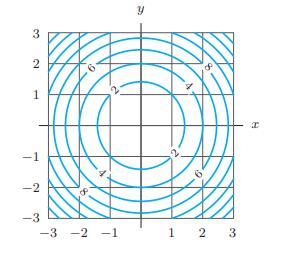
\includegraphics[scale=0.7,alt={contour plot of concentric circles about the origin increasing in value with distance from the origin}]{contour_14_5.png}
	\end{minipage}
	\begin{minipage}{0.6\linewidth}	
		\begin{enumerate}
			\item At the point $(-2,2)$ in the direction $\bi$
			\item At the point $(0,-2)$ in the direction $\bj$
			\item At the point $(-1,1)$ in the direction $\bi +\bj$
			\item At the point $(-1,1)$ in the direction $-\bi+\bj$
			\item At the point $(0,-2)$ in the direction $\bi - 2\bj$
		\end{enumerate}
	\end{minipage}}
    { % answer goes here
	\begin{enumerate}
			\item Negative
			\item Negative
			\item Approximately zero
			\item Positive
			\item Positive
		\end{enumerate}
	}
	{ % solution goes here
	}

	\item \question{
	Let $f(x,y)=-x^2y+xy^2+xy$ and $P=(2,1)$.
	\begin{enumerate}
		\item Find the direction of maximal increase of $f$ at $P$.
		\item What is the maximum rate of change of $f$ at $P$?
		\item Find the direction of maximal decrease of $f$ at $P$.
		\item Find a direction $\bu$ such that $D_{\bu}f(P)=0$ (note this forces $\bu$ to be a unit vector!).
	\end{enumerate}}
	{ % answer goes here
		\begin{enumerate}
			\item $\langle -1/\sqrt{2},1/\sqrt{2} \rangle$
			\item $2\sqrt{2}$
			\item $\langle 1/\sqrt{2},-1/\sqrt{2} \rangle$
			\item $\langle 1/\sqrt{2},1/\sqrt{2} \rangle$
		\end{enumerate}
	}
	{ % solution goes here
	}
\end{enumerate}


% 
\fancyhead[C]{Section 14.6}
\fancyhead[R]{\daytwelve}

\iftoggle{questions}{
\begin{center}{\large \textbf{Math 2551 Worksheet: Linearization and Tangent Planes}}
\end{center}

\begin{enumerate}
	\item %14.6 # 30b
	Find the linearization of $f(x,y)=e^{2y-x}$ at $(1,2)$. 
	
	\item Find the linearization of $f(x,y,z)=\tan^{-1}(xyz)$ at $(1,1,0)$.
	\item Use the linearization to approximate $f(2.95, 7.1)$ for the function $f(x,y)=\sqrt{x^2+y}$, knowing that $f(3,7)=4$.	
	
	
	\item Graph the function $z=x^{1/3}y^{1/3}$.  Examine the graph at $(0,0)$ - does it look like the function can be well-approximated by a tangent plane there?  Based on your conclusion, is this function differentiable at $(0,0)$?
	
	\item Find the equation for the plane tangent to the graph of $f(x,y)=\sqrt{y-x}$ when $x=1$ and $y=2$.
\end{enumerate}
}{}

\iftoggle{answers}{
\begin{center}{\large \textbf{Math 2551 Worksheet Answers: Linearization and Tangent Planes, Optimization}}
\end{center}

\begin{enumerate}
		\item $L(x,y)=e^3-e^3(x-1)+2e^3(y-2)$
	\item $L(x,y,z)=z$
	
	\item $f(2.95, 7.1)=4-1/40$
	
	\item No, there are two different tangent planes.  No, the function is not differentiable.
	
	\item $z=1-1/2(x-1)+1/2(y-2)$
	
\end{enumerate}
}{}
\iftoggle{solutions}
{
Solutions go here in the same format.
}{}

% \fancyhead[C]{Section 14.7}
\fancyhead[R]{\daytwelve/\daythirteen}

\section*{\centering Chapter 14.7: Optimization}

\textbf{D3: Optimization.} I can locate and classify critical points of functions of two variables. I can find absolute maxima and minima on closed bounded sets. I can use the method of Lagrange multipliers to maximize and minimize functions of two or three variables subject to constraints. I can interpret the results of my calculations to solve problems.

\subsection*{Mechanics}
\begin{enumerate}	
	\item \question{Find and classify all critical points for the function $x^3+3xy+y^3$.}
    {% answer goes here
        Saddle point at $(0,0)$ and local minimum at $(0,-2)$.
    }
    {% solution goes here
    } 
    \item \question{Find all the local maxima, local minima, and saddle points of $f(x,y) = e^y(x^2-y^2)$. }
    {% answer goes here
        Saddle point at $(0,0)$ and local maximum at $(-1,-1)$.
    }
    {% solution goes here
    } 
    \item \question{Find the absolute maxima and minima of the function $f(x,y)=x^2-xy+y^2+1$ on the closed triangular plate bounded by lines $x=0$, $y=4$, $y=x$ in the first quadrant.}
    {% answer goes here
        The absolute maximum is $17$, achieved at $(0,4)$ and $(4,4)$, and the absolute minimum is $1$, achieved at $(0,0)$.
    }
    {% solution goes here
    } 
    \item \question{Give an example of a differentiable function $f(x,y)$ with no critical points.}
    {% answer goes here
        Many possible examples, e.g. any linear function $f(x,y)=ax+by+c$.
    }
    {% solution goes here
    } 
\end{enumerate}
\subsection*{Applications}
\begin{enumerate}[resume]
\item \question{A terrible recipe for lemonade calls for you to just mix lemon juice, denoted by $\ell$, and
water, denoted by $w$ (units in tonnes). Suppose that given a pair $(\ell,w)$, you are able to
make $f(\ell,w) = \ell^2-\ell w + w$ liters of lemonade. Given that have only 2 tonnes of lemon juice and 3 tonnes of water, what is the maximum amount of (a very acidic) lemonade
can you make? How much of each ingredient is used?}
    { $f_{max} = 4$ is the unique maximum attained at $(\ell,w) = (2,0)$. This means that the lemonade is pure lemon juice :)
    }
    {% solution goes here
    } 
\item \question{
In an alternate universe, Atlanta is famous for her extravagant beaches and pristine waters. In this universe, it is known that Atlanta's waters are extremely wavy, and the height of the water (relative to ground level) may be modeled by the function $h(x,y)=\sin(x)\cos(y)$, for $x\in (0,2\pi)$ and $y\in (0,2\pi)$. Visualize this using a 3D graphing software, and compute the height of the highest tides as well as the depth of the lowest troughs. At which coordinates $(x,y)$ do these tides and troughs occur?
}
    {% answer goes here
    Highest tides are at $1$ occurring at $(3\pi/2,\pi)$, lowest troughs at $-1$ occurring at $(\pi/2,\pi)$.
    }
    {% solution goes here
    }
    \item \question{Let us interpret local maxima as peaks of mountains, local minima as valleys and saddle points as passes between mountain peaks. Consider the statement: ``It is impossible to have two mountain peaks without some sort of valley or pass connecting them. Therefore, if a function has two local maxima, there must also be a saddle point or a local minimum." Do you agree with this? Verify your answer by using software to graph the function $f(x,y)=4x^2e^y-2x^4-e^4y$.} 
	{% answer goes here
    The statement is false! The function given has precisely two local maximums and no other critical points. 
    }
    {% solution goes here
    } 
\end{enumerate}
\subsection*{Extensions}
\begin{enumerate}[resume]	
	\item \question{Can you conclude anything about $f(a, b)$, if $f$ and its first and second partial derivatives are continuous around the critical point $(a, b)$ and $f_{xx}(a,b)$ and $f_{yy}(a,b)$ have opposite signs? 
    Justify your answer.}
    {% answer goes here
        Yes, this must be a saddle point because $f_{xx}(a,b)f_{yy}(a,b)<0$ so $\det(Hf)=f_{xx}(a,b)f_{yy}(a,b)-f_{xy}^2(a,b)<0$.
    }
    {% solution goes here
        Yes, this must be a saddle point because $f_{xx}(a,b)f_{yy}(a,b)<0$ so $\det(Hf)=f_{xx}(a,b)f_{yy}(a,b)-f_{xy}^2(a,b)<0$.
    } 
    
	\item \question{In each case, the origin is a critical point of $f$ and $f_{xx}f_{yy}-(f_{xy})^2 = 0$ at the origin, so the Second Derivative Test fails at the origin.  
    Use some other method to determine whether the function $f$ has a maximum, a minimum, or neither at the origin.
	\begin{enumerate}
		\item $f(x,y)= x^2y^2$
		\item $f(x,y)= 1-x^2y^2$
		\item $f(x,y)= xy^2$
		\item $f(x,y)= x^3y^2$
		\item $f(x,y)= x^3y^3$
		\item $f(x,y)= x^4y^4$
	\end{enumerate}}
    {% answer goes here
    \begin{enumerate}
		\item Minimum is $0$ at $(0,0)$ since $f(x,y)>0$ for all other $(x,y)$.
		
		\item Maximum is $1$ at $(0,0)$ since $f(x,y)<1$ for all other $(x,y)$.
		
		\item Neither since $f(x,y)<0$ for $x<0$ and $f(x,y)>0$ for $x>0$.
		
		\item Neither since $f(x,y)<0$ for $x<0$ and $f(x,y)>0$ for $x>0$.
		
		\item Neither since $f(x,y)<0$ for $x<0$ and $y>0$, but $f(x,y)>0$ for $x>0$ and $y>0$.
		
		\item Minimum is $0$ at $(0,0)$ since $f(x,y)>0$ for all other $(x,y)$.
	\end{enumerate}
    }
    {% solution goes here
    \begin{enumerate}
		\item Minimum is $0$ at $(0,0)$ since $f(x,y)>0$ for all other $(x,y)$.
		
		\item Maximum is $1$ at $(0,0)$ since $f(x,y)<1$ for all other $(x,y)$.
		
		\item Neither since $f(x,y)<0$ for $x<0$ and $f(x,y)>0$ for $x>0$.
		
		\item Neither since $f(x,y)<0$ for $x<0$ and $f(x,y)>0$ for $x>0$.
		
		\item Neither since $f(x,y)<0$ for $x<0$ and $y>0$, but $f(x,y)>0$ for $x>0$ and $y>0$.
		
		\item Minimum is $0$ at $(0,0)$ since $f(x,y)>0$ for all other $(x,y)$.
	\end{enumerate}
    } 
    \item \question{Among all rectangular boxes of volume $27$ cm$^3$, what are the dimensions of the box with the smallest surface area?  
    What is the smallest possible surface area? (you may assume this occurs at a local min of the surface area function)}
    {% answer goes here
        The dimensions are $3 \times 3 \times 3$ and the surface area is $54$.
    }
    {% solution goes here
    } 
    
	
\end{enumerate}

% 
\fancyhead[C]{Section 14.7}
	\fancyhead[R]{\daythirteen}
\iftoggle{questions}{
\begin{center}{\large \textbf{Math 2551 Worksheet: Optimization II}}
\end{center}


\begin{enumerate}
	\item Find the absolute maxima and minima of the function $f(x,y)=x^2-xy+y^2+1$ on the closed triangular plate bounded by lines $x=0$, $y=4$, $y=x$ in the first quadrant.
	
	\item Among all rectangular boxes of volume $27$ cm$^3$, what are the dimensions of the box with the smallest surface area?  What is the smallest possible surface area?  (assume this occurs at a local min of the surface area function)
	
\end{enumerate}
}{}

\iftoggle{answers}{
\begin{center}{\large \textbf{Math 2551 Worksheet Answers: Optimization II}}
\end{center}

\begin{enumerate}

	\item The absolute maximum is $17$, achieved at $(0,4)$ and $(4,4)$, and the absolute minimum is $1$, achieved at $(0,0)$.
	
	\item The dimensions are $3 \times 3 \times 3$ and the surface area is $54$.
	
\end{enumerate}
}{}
\iftoggle{solutions}
{
Solutions go here in the same format.
}{}

% 
\fancyhead[C]{Section 14.8}
\fancyhead[R]{\daythirteen}

\section*{\centering Chapter 14.8: Lagrange Multipliers}

\textbf{D3: Optimization.} I can locate and classify critical points of functions of two variables. I can find absolute maxima and minima on closed bounded sets. I can use the method of Lagrange multipliers to maximize and minimize functions of two or three variables subject to constraints. I can interpret the results of my calculations to solve problems.

\subsection*{Mechanics}
\begin{enumerate}	
	\item \question{Find the extreme values of the function $f(x,y)=x^2+2y^2$ on the circle $x^2+y^2=1$.}
	%1, 2}
    {% answer goes here
    The extreme values are 1 and 2.
    }
    {% solution goes here
    } 
    \item \question{Find the extreme values of the function $f(x,y,z)=x^2+y^2+z^2$ subject to the constraint $x^4+y^4+z^4=1$.}
    {% answer goes here
    The extreme values are 1 and $\sqrt{3}$.
    }
    {% solution goes here
    } 

\end{enumerate}
\subsection*{Applications}
\begin{enumerate}[resume]
    \item \question{A rectangular box without a lid is to be made from 12 $m^2$ of cardboard. Find the maximum volume of such a box.}  %(2,2,1)
    {% answer goes here
    $V(2,2,1)=4$ cubic units
    }
    {% solution goes here
    } 
    \item \question{A niche restaurant in midtown Atlanta serves only garlic bread (denoted by $g$) and bunches of kale (denoted by $k$). The cost of producing these goods is given by the function $C(g,k) = 5g^2+2gk+3k^2+10$. Assuming that the total amount of items to be produced is 40, compute the minimal production cost.}
    {% answer goes here
    $ C_{min}=\frac{11230}{3} \approx \$3743.33$.
    }
    {% solution goes here
    } 
    \item \question{The height of a mountain is given by $h(x,y)= 300-(3x^2+4xy+3y^2)$. Compute the height of the lowest point on the mountain within $\sqrt{200}$ units of the origin. Where might this point occur? Are there multiple points where this occurs? \textit{[Hint: First, justify why none of $x,y,\lambda$ can be zero. Then solve for $\lambda$.}]}
    {% answer goes here
    The two minimums occur at $(x,y)= (\pm 10,\pm 10)$, where the height is -700 units. Warning: The two other solutions to the Lagrange system are $(x,y)=(\pm 10,\mp 10)$ and they are maximums at height 100.
    }
    {A routine check shows that the only critical point is at $(0,0)$, which is not a minimum by the second derivative test. Therefore, we check on the boundary $x^2+y^2 = 200$. The Lagrange system looks like 
    \begin{align*}
        -6x-4y &= 2\lambda x\\
        -4x-6y &= 2\lambda y\\
        x^2+y^2 &= 200
    \end{align*}
    Note that if either $x,y$ or $\lambda$ is zero, at least one of the three equations will be violated, hence we are free to divide at leisure. Solving for $\lambda$ in two different ways and equating gives us $x/y = y/x$. Plugging into the constraint equation yields that $x=\pm 10$ and $y=\pm 10$. A routine check distinguishes two of these as maximums and two as minimums.  
    } 
\end{enumerate}
\subsection*{Extensions}
\begin{enumerate}[resume]
    \item \question{The plane $x+y+2z=2$ intersects the paraboloid $z=x^2+y^2$ in an ellipse.  Find the points on this ellipse that are nearest to and farthest from the origin. \textit{[Hint: It may be helpful algebraically to work with the square of the distance to the origin.]}}
    {% answer goes here
    The closest point is $(\dfrac{1}{2},\dfrac{1}{2},\dfrac{1}{2})$ and the farthest point is $(-1,-1,2)$.
    }
    {% solution goes here
    } 

	
	\item \question{Find the maximum volume of a rectangular box that is inscribed in a sphere of radius $r$.}
    {% answer goes here
    $\dfrac{8r^3}{3\sqrt{3}}$
    }
    {% solution goes here
    } 
    
\end{enumerate}
% 
\fancyhead[C]{Section 15.1}
\fancyhead[R]{\dayfifteen}

\section*{\centering Chapter 15.1: Double Integrals on Rectangles}
\textbf{I1: Double \& Triple Integrals.} I can set up double and triple integrals as iterated integrals over any region. I can sketch regions based on a given iterated integral.\\\\
\textbf{I2: Iterated Integrals.} I can compute iterated integrals of two and three variable functions, including applying Fubini's Theorem to change the order of integration of an iterated integral.

\subsection*{Mechanics}
\begin{enumerate}
    \item \question{Compute $\displaystyle \iint_R (xy-3xy^2) \ dA$, where  $R$ is the square $0 \leq x \leq 2,1 \leq y \leq 2$.}{-11
    }
    {% solution goes here
    } 
    \item \question{Use Fubini's Theorem to evaluate the integral
	\begin{equation*}
	    \int_0^1 \int_0^3 xe^{xy}\ dx\ dy 
	\end{equation*} 
    Why was it a good idea to exchange the order of integration?}{% answer goes here
    }
    {% solution goes here
    } 
    \item \question{Find the volume of the region bounded above by the paraboloid $z = 16 - x^2 - y^2$ and below by the square 
$R: 0 \leq x \leq 2, 0 \leq y \leq 2$.}{% answer goes here
    }
    {% solution goes here
    } 
\end{enumerate}
\subsection*{Extensions}
\begin{enumerate}[resume]
\item \question{Evaluate the double integral $\iint_R (4-2y)\ dA$, where $R=[0,1]\times[0,1]$ \textbf{without integrating} by identifying it as the volume of a solid \textit{[Hint: It is a prism cut by some plane.]}}{% answer goes here
    }
    {% solution goes here
    } 

\item \question{The integral $\iint_R \sqrt{9-y^2}$, where $R=[0,4]\times[0,2]$, represents the volume of a solid.  Sketch the solid.}{% answer goes here
    }
    {% solution goes here
    } 
	
	\item \question{This problem explores a failure of Fubini's theorem. Consider the two iterated integrals, which differ by swapping the order of integration:
	\begin{equation*}
	\int_0^1 \int_0^1 \frac{x^2-y^2}{(x^2+y^2)^2}\ dy\ dx \quad \textrm{ and }\quad \int_0^1 \int_0^1 \frac{x^2-y^2}{(x^2+y^2)^2}\ dx\ dy \end{equation*}
    Use the fact that 
    \begin{equation*}
        \frac{\partial}{\partial y} \left(\frac{y}{x^2+y^2}\right)=\frac{\partial}{\partial x} \left(\frac{-x}{x^2+y^2}\right)= \frac{x^2-y^2}{(x^2+y^2)^2}
    \end{equation*}
    and that $\frac{d}{dt}\arctan(t) = 1/(1+t^2)$ to show that the iterated integrals are different. Why does Fubini's theorem fail? }
    {% answer goes here
    }
    {% solution goes here
    } 
	
\end{enumerate}
{}

\iftoggle{answers}{
\begin{center}{\large \textbf{Math 2551 Worksheet Answers: Double Integrals on Rectangles}}
\end{center}

\begin{enumerate}
	\item 
	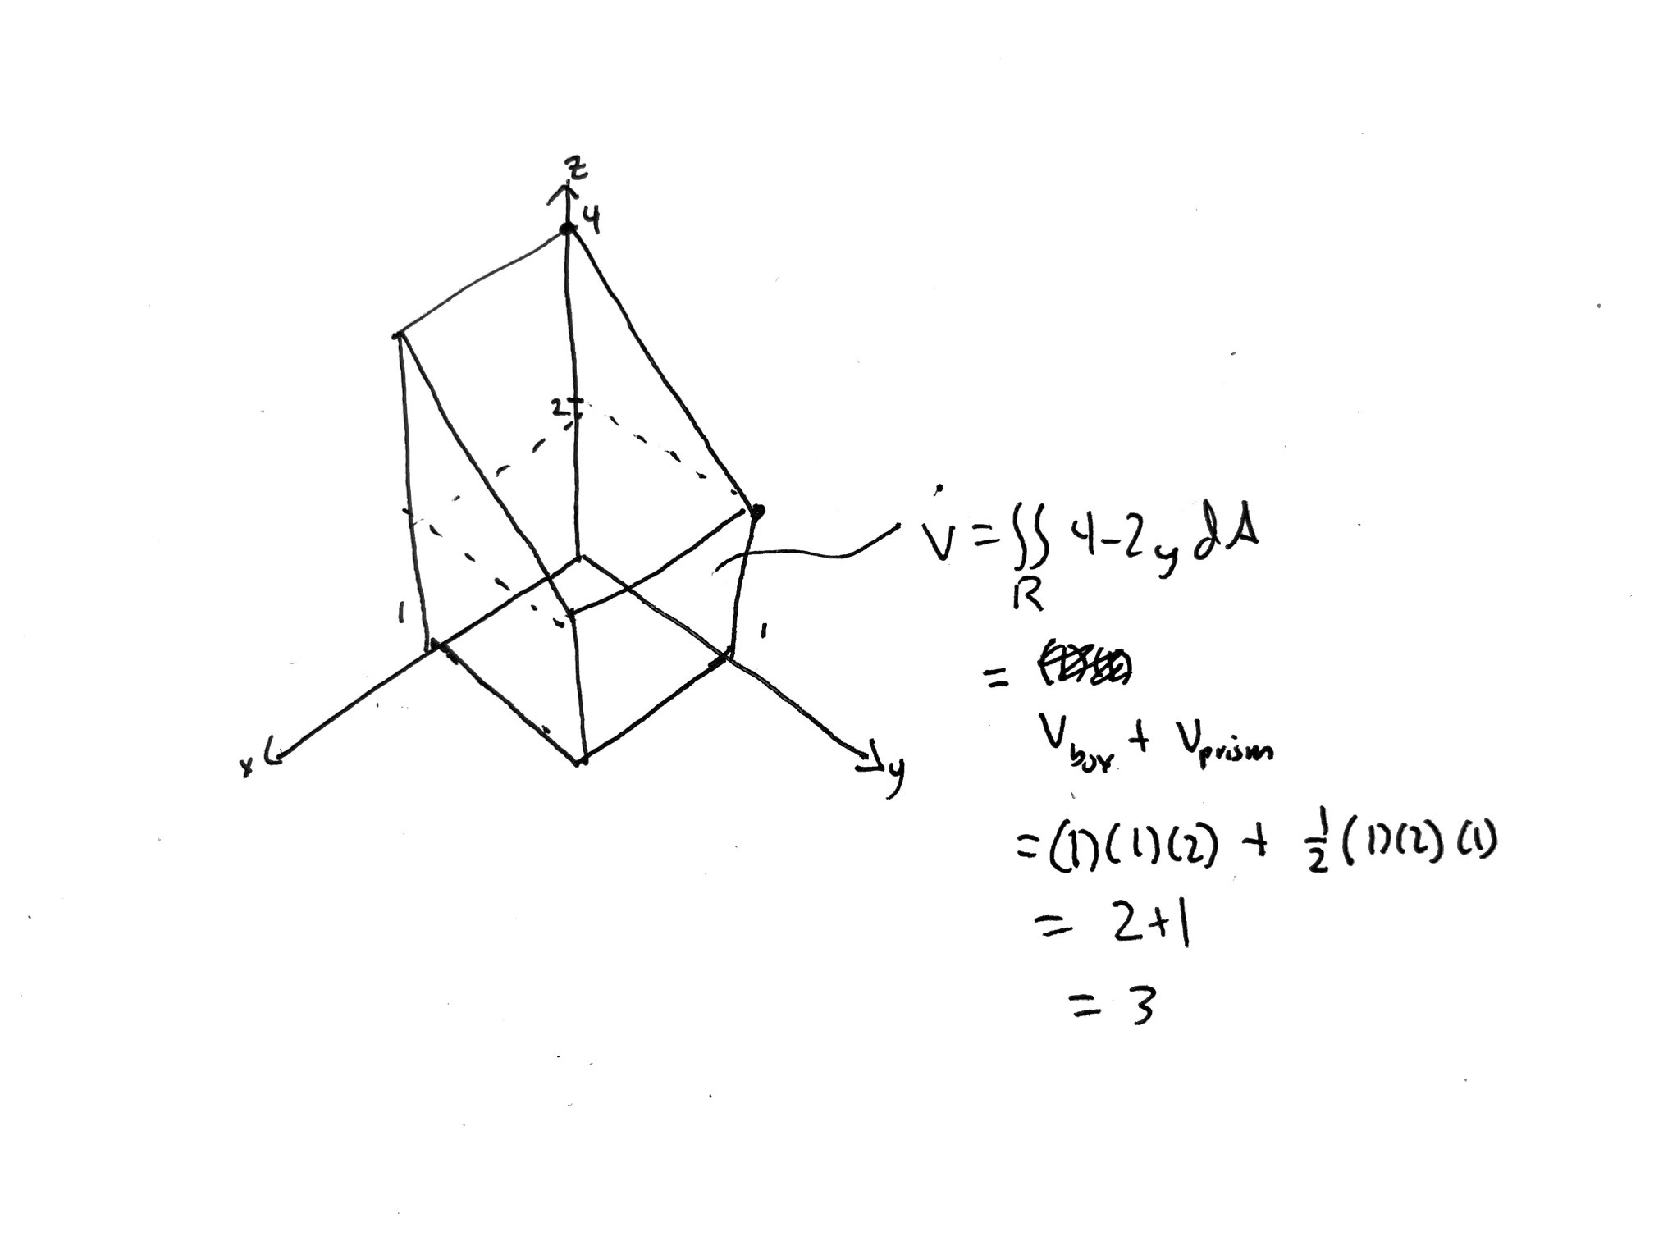
\includegraphics[scale=0.3]{ws_15_1_src.pdf}
	
	\item 
	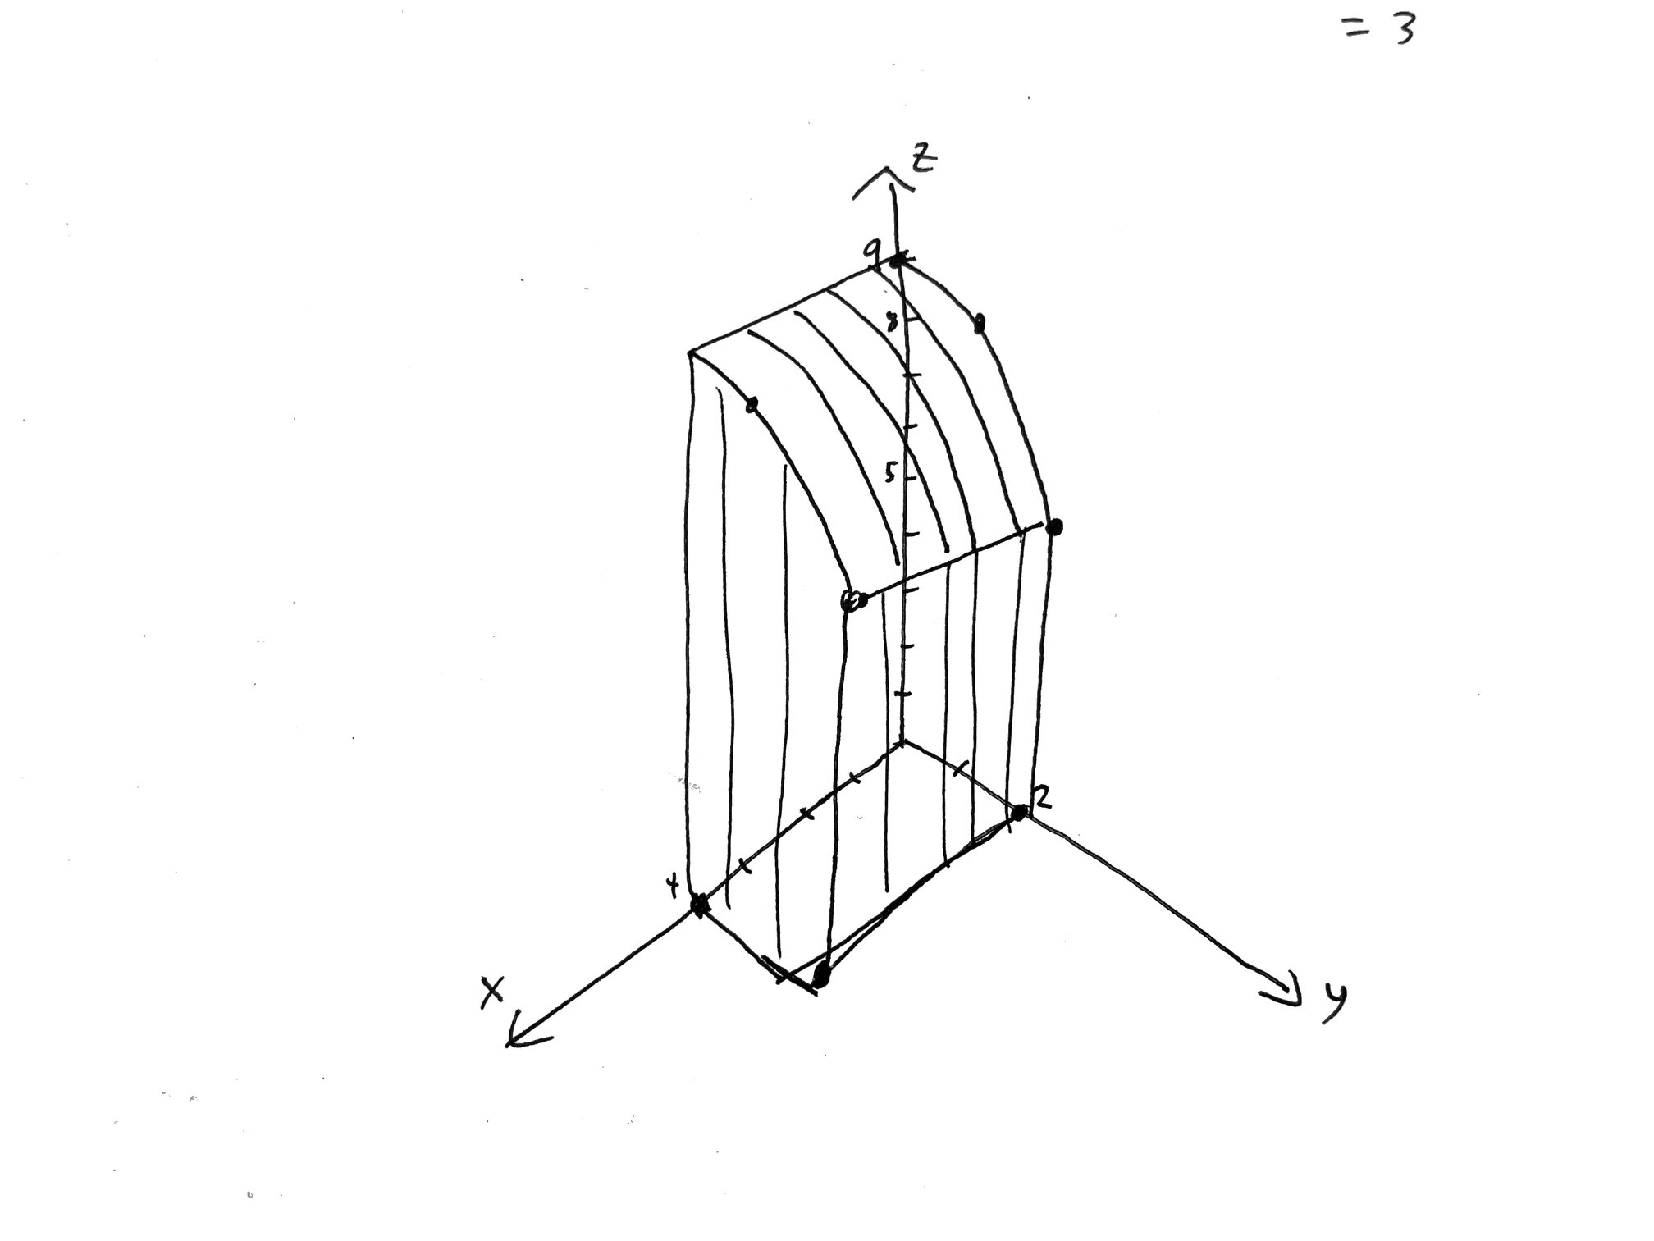
\includegraphics[scale=0.25]{ws_15_2_src.pdf}
	
	\item $9\ln(2)$
	
	\item $160/3$ cubic units.
	
		\item $e^3-4$

	\item The integrals evaluate to $\pi/4$ and $-\pi/4$ respectively.  This does not violate Fubini's theorem because this function is not continuous on $[0,1]\times[0,1]$ (it has an asymptote at $(0,0)$)
\end{enumerate}
}{}
\iftoggle{solutions}
{
Solutions go here in the same format.
}{}

% \fancyhead[C]{Section 15.2}
	\fancyhead[R]{\dayfifteen}
	
\iftoggle{questions}{
\begin{center}{\large \textbf{Math 2551 Worksheet: Double Integrals on General Regions}}
\end{center}

\begin{enumerate}

\item Compute the integrated integral
\[\int_0^\pi \int_0^x x \sin (y)\ dy\ dx. \]


\item Decide, without calculation, if each of the integrals below are positive, negative, or zero. Let D be the region inside the unit circle centered at the origin. Let T, B, R, and L denote the regions enclosed by the top half, the bottom half, the right half, and the left half of unit circle, respectively.

\begin{multicols}{2}
	\begin{enumerate}
		\item $\iint_B (y^3+y^5)\ dA$
		\item $\iint_T (y^3+y^5)\ dA$
		\item $\iint_D (y^3+y^5)\ dA$
		\item $\iint_L (y^3+y^5)\ dA$
		\item $\iint_R (y^3+y^5)\ dA$
	\end{enumerate}
\end{multicols}

\item Write an iterated integral for $\iint_R 1 \ dA$ over the region $R$ using vertical cross-sections and horizontal cross-sections. 
\begin{enumerate}
	\item Bounded by $y=e^{-x}$, $y=1$, and $x=\ln 3$.
	
	\item Bounded by $y=x^2$ and $y=x+2$
\end{enumerate}

	\item Sketch the region of integration, reverse the order of integration, and evaluate the integral.
	\[\displaystyle \int_0^{\sqrt{\pi}} \int_y ^{\sqrt{\pi}} \cos(x^2) \ dx \ dy.\]
	\item Sketch the region of integration and evaluate the integral \[ \iint_R xy^2\ dA, \] where $R$ is enclosed by $x=0$ and $x=\sqrt{1-y^2}$.
	
	
	\item Find the volume of the solid bounded by the cylinder $y^2+z^2=4$ and the planes $x=2y$, $x=0$, $z=0$ in the first octant.
	
	\item The integral expression below gives the area of a region in the $xy$-plane. Sketch the region, labeling the bounding curves with their equations, and giving the coordinates of points where the curves intersect.  Then find the area of the region.
	\[ \int_0^2 \int_{x^2-4}^0\ dy\ dx + \int_0^4\int_{0}^{\sqrt{x}}\ dy\ dx \]
	
	
\end{enumerate}
}{}

\iftoggle{answers}{
\begin{center}{\large \textbf{Math 2551 Worksheet Answers: Double Integrals on General Regions}}
\end{center}

\begin{enumerate}
	
	\item $2+\frac{1}{2}\pi^2$
	
	\item \begin{enumerate}
		\item Negative
		\item Positive
		\item Zero
		\item Zero
		\item Zero
	\end{enumerate}
	
	
	\item \begin{enumerate}
		\item $\int_0^{\ln(3)} \int_{e^{-x}}^1\ dy\ dx$ and $\int_{1/3}^1 \int_{-\ln(y)}^{\ln(3)}\ dx\ dy$
		
		\item $\int_{-1}^2 \int_{x^2}^{x+2} \ dy\ dx$ and $\int_0^1 \int_{-\sqrt{y}}^{\sqrt{y}} \ dx\ dy + \int_1^4 \int_{y-2}^{\sqrt{y}}\ dx\ dy$
	\end{enumerate}
	\item $ \int_0^{\sqrt{\pi}} \int_0^{x} \cos(x^2) \ dy \ dx=0$
	\item $\dfrac{2}{15}$
	
	
	\item $16/3$
	
	\item $32/3$	
\end{enumerate}
}{}
\iftoggle{solutions}
{
Solutions go here in the same format.
}{}

% 
\fancyhead[C]{Section 15.3}
\fancyhead[R]{\dayfifteen}

\section*{\centering Chapter 15.3: More Double Integrals}
\textbf{I1: Double \& Triple Integrals.} I can set up double and triple integrals as iterated integrals over any region. I can sketch regions based on a given iterated integral.

\textbf{I2: Iterated Integrals.} I can compute iterated integrals of two and three variable functions, including applying Fubini's Theorem to change the order of integration of an iterated integral.

\subsection*{Mechanics}
\begin{enumerate}
    	\item \question{
         Consider the function $f(x,y)=xy$. Without performing any computations, do you think the average value of $f$ is larger over the square $0\leq x \leq 1, 0\leq y\leq 1$, or over the quarter circle $x^2+y^2\leq 1$ \textit{in the first quadrant}? Verify your guess by integrating
        }
        {% answer here
        
        }
        {% solution here
        
        }
       
        \item \question{
        A metal triangular plate with vertices $(0,0)$, $(2,0)$ and $(2,4)$ has temperature equal to $C(x,y) = xe^{xy}$ degrees Celsius. Compute the average temperature of the plate. \textit{[Hint: Choose a favourable order of integration.]}
        }
        {% answer here
        
        }
        {% solution here
        
        }
\end{enumerate}
\subsection*{Applications}
\begin{enumerate}[resume]
    \item \question{
        If $f(x,y)=100(y+1)$ represents the population density in people per square mile of a planar region on Earth, where $x$ and $y$ are measured in miles, find the number of people in the region bounded by the curves $x=y^2$ and $x=2y-y^2$.
        }
        {% answer here
        
        }
        {% solution here
        
        }
    \item \question{
        A rectangular can of Pringles chips may be modelled by the prism $0\leq x \leq 1$, $0\leq y \leq 1$ and $0\leq z\leq 5$. Assuming that the Pringles container is filled up with chips until the surface $z=x^2-y^2+3$, are there more chips or air in the can? \textit{[Note: The Pringles enthusiast may complain that their containers are supposed to be cylinders, not prisms. This nuance will be addressed when we work with polar coordinates.]}
        }
        {% answer here
        
        }
        {% solution here
        
        }
\end{enumerate}
\subsection*{Extensions}
\begin{enumerate}[resume]
	\item \question{
        An organism can be initially described as the solid with base $[0,1]\times [0,1]$ and height $z = e^{x+y}$. Suppose that the base of this organism grows at a rate of $t$ units per second in both the positive $x$ and positive $y$ directions. Compute the rate of change of the volume of the organism at $t=4$ seconds. \textit{[Hint: Set up an integral expression for the volume in terms of $t$, evaluate the integral, then differentiate with respect to $t$.]}
        }
        {% answer here
        
        }
        {% solution here
        
        }
	
\end{enumerate}
{}

\iftoggle{answers}{
\begin{center}{\large \textbf{Math 2551 Worksheet 16 Answers: Applications, Polar Double Integrals}}
\end{center}

\begin{enumerate}
	\item Answers will vary a bit through the estimation process
	
	4 subdivisions: $31.75 \leq T_{avg} \leq 52.5$\\
	16 subdivisions: $33.18  \leq T_{avg} \leq 50.06$\\
	25 subdivisions: $36.32  \leq T_{avg} \leq 49.8$\\
	
	Colorado is a rectangle, which makes it easy to subdivide. Wyoming would also work well.
	
	
	\item On square: $f_{avg}=\frac{1}{1}\cdot \frac{1}{4}=\frac{1}{4}$\\
	
	On quarter circle: $f_{avg}=\frac{1}{\pi/4}\cdot \frac{1}{8}=\frac{1}{2\pi}$ 
	\item 50 people
\end{enumerate}
}{}
\iftoggle{solutions}
{
Solutions go here in the same format.
}{}
% 
\fancyhead[C]{Section 15.4}
\fancyhead[R]{\daysixteen}

\section*{\centering Chapter 15.4: Polar Coordinates}
\textbf{I3: Change of Variables.} I can use polar, cylindrical, and spherical coordinates to transform double and triple integrals and can sketch regions based on given polar, cylindrical, and spherical iterated integrals. I can use general change of variables to transform double and triple integrals for easier calculation.  I can choose the most appropriate coordinate system to evaluate a specific integral.

\subsection*{Mechanics}
\begin{enumerate}
\item \question{
        Use polar coordinates to compute the integral:
	\begin{equation*}
	\int_{0}^{2}\int_{-\sqrt{4-y^2}}^{\sqrt{4-y^2}} e^{-x^2-y^2} \ dx \ dy
	\end{equation*}
        }
        {% answer here
        
        }
        {% solution here
        
        }
    
	\item \question{
        Evaluate $\displaystyle \iint_D y^2+3x\ dA$ where $D$ is the region in the 3rd quadrant between $x^2+y^2=1$ and $x^2+y^2=9$.
        }
        {% answer here
        
        }
        {% solution here
        
        }
	
	\item \question{
        Use a double integral to determine the volume of the solid that is inside the cylinder $x^2+y^2=16$, below $z=2x^2+2y^2$, and above the $xy$-plane.
        }
        {% answer here
        
        }
        {% solution here
        
        }
    \item \question{
        Give an example of region and function you would \textit{not} want to use polar coordinates to integrate. Justify your answer. 
        }
        {% answer here
        
        }
        {% solution here
        
        }
\end{enumerate}
\subsection*{Applications}
\begin{enumerate}[resume]
    \item \question{
        The previous worksheet featured a problem involving a peculiar Pringles can. This problem rectifies that inconsistency.
    
    A true can of Pringles chips may be modeled by the cylinder $x^2+y^2=1$ bounded above and below like $0\leq z\leq 5$. Assuming that the Pringles container is filled up with chips until the surface $z=x^2-y^2+3$, are there more chips or air in the can? \textit{[Hint: Use the identity $\cos^2\theta-\sin^2\theta = \cos 2\theta$].}
        }
        {% answer here
        
        }
        {% solution here
        
        }
    
    \item \question{
        In the town of Churchill in northern Canada, the density of polar bears around the town dump is given by $p(x,y)=e^{x^2+y^2}$ bears per square unit. Use polar coordinates to compute the average number of polar bears in the region $1\leq x^2+y^2\leq 2 $.
        }
        {% answer here
        
        }
        {% solution here
        
        }
\end{enumerate}
\clearpage

\subsection*{Extensions}
\begin{enumerate}[resume]	
	\item \question{
        Find the area of the region common to the interiors of the cardioids $r=1+\cos \theta$ and $r=1-\cos \theta$. \textit{[Hint: Use symmetry to restrict your calculation to only the first quadrant.]}
	
	\begin{center}
		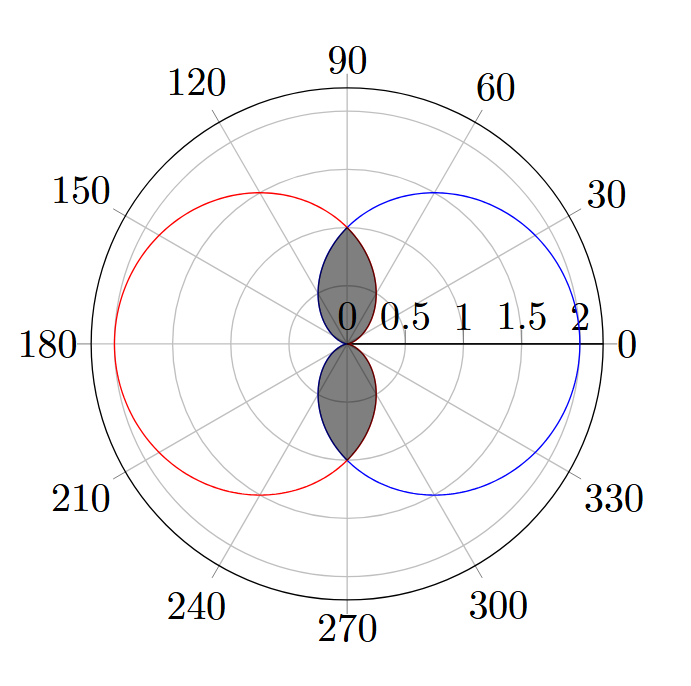
\includegraphics[scale=0.4,alt={plot of the double-teardrop shaped region between the two cardioids specified above, with intersection points at (r,theta)=(0,0),(1,pi/2),(1,3pi/2)}]{ws_15_4_cardioids.png}
	\end{center}
        }
        {% answer here
        
        }
        {% solution here
        
        }
	
	\item \question{
        An integral of great importance in statistics is the Gaussian integral $I=\Ds \int_0^\infty e^{-x^2}\ dx$.  The function $f(x)=e^{-x^2}$ has no elementary antiderivative, so this integral is hard to compute in the usual way. Fortunately, polar coordinates provide a solution.
	
	Notice that $I^2=\Ds \left(\int_0^\infty e^{-x^2}\ dx\right)\left(\int_0^\infty e^{-y^2}\ dy\right) = \int_0^\infty \int_0^\infty e^{-x^2-y^2}\ dxdy $.
	
	\begin{enumerate}
		\item The domain of the above double integral is the first quadrant $[0,\infty)\times [0,\infty)$. Describe this region using polar coordinates, and transform $I^2$ into an (improper) polar integral. 
		
		\item Evaluate your double integral to compute the value of $I^2$.  Use this to find the value of the original Gaussian integral $I$.
	\end{enumerate}

	You can find some history of this integral \href{https://www.york.ac.uk/depts/maths/histstat/normal_history.pdf}{here}.
        }
        {% answer here
        
        }
        {% solution here
        
        }
	
\end{enumerate}
{}

\iftoggle{answers}{
\begin{center}{\large \textbf{Math 2551 Worksheet Answers: Polar Double Integrals}}
\end{center}

\begin{enumerate}
	\item $5\pi-26$
	
	\item $\dfrac{\pi}{2}(1-e^{-4}).$
	
	\item $\dfrac{3\pi}{2}-4$.
	
	\item $256\pi$
	
	\item \begin{enumerate}
		\item $I^2=\Ds \lim_{R\to\infty}\int_0^2\pi\int_0^R e^{-r^2}r\ dr\ d\theta$
		
		\item $I^2=\dfrac{\pi}{4}$, so $I=\dfrac{\sqrt{\pi}}{2}$
	\end{enumerate}
\end{enumerate}
}{}
\iftoggle{solutions}
{
Solutions go here in the same format.
}{}
% \fancyhead[C]{Sections 14.3-14.8, 15.1-15.4}
	\fancyhead[R]{\dayseventeen}

\iftoggle{questions}{
\begin{center}{\large \textbf{Math 2551 Worksheet: Exam 2 Review}}
\end{center}


\begin{enumerate}
	
	
	\item Which of the following statements are true if $f(x, y)$ is differentiable
	at $(x_0 , y_0)$? Give reasons for your answers.
	\begin{enumerate}
		\item  If $\bu$ is a unit vector, the derivative of $f$ at $(x_0 , y_0)$ in the direction
		of $\bu$ is $(f_x(x_0 , y_0)\bi + f_y(x_0 , y_0)\bj) \cdot \bu$.
		\item The derivative of $f$ at $(x_0 , y_0)$ in the direction of $\bu$ is a vector.
		\item The directional derivative of $f$ at $(x_0 , y_0)$ has its greatest value
		in the direction of $\nabla f$.
		\item At $(x_0 , y_0)$, the vector $\nabla f$ is normal to the curve $f(x, y) = f(x_0 , y_0)$.
	\end{enumerate}
	
	\item Find $dw/dt$ at $t = 0$ if $w = \sin(xy + \pi), x = e^t,$ and $y =
	\ln(t + 1).$
	
	\item Find the extreme values of $f(x, y) = x^3 + y^2$ on the circle $x^2 + y^2 = 1$.
	
	\item Test the function $f(x,y)=x^3+y^3+3x^2-3y^2$ for local maxima and minima and saddle points and find the function's value at these points.
	
	\item Find the points on the surface $xy+yz+zx-x-z^2=0$ where the tangent plane is parallel to the $xy$-plane.
	
	\item Evaluate the integral $\displaystyle \int_0^1\int_{2y}^2 4\cos(x^2)\ dx\ dy$. Describe why you made any choices you did in the course of evaluating this integral.
	
	\item If $f(x,y)\geq 2$ for all $(x,y)$, is it possible that the average value of $f(x,y)$ on a unit disk centered at the origin is $\dfrac{2}{\pi}$?
	
	\item A swimming pool is circular with a 40 foot diameter.  The depth is constant along east-west lines and increases linearly from 2 feet at the south end to 7 feet at the north end.  Find the volume of water in the pool.
	
\end{enumerate}
}{}

\iftoggle{answers}{
\begin{center}{\large \textbf{Math 2551 Worksheet Answers: Exam 2 Review}}
\end{center}

\begin{enumerate}
	
	\item All are true except b).
	
	
	\item -1
	
	\item $\pm 1$
	
	\item Saddle at $(0,0)$ with $f(0,0)=0$, local min at $(0,2)$ of $-4$, local max at $(-2,0)$ of 4, saddle at $(-2,2)$ with $f(-2,2)=0$
	
	\item $(-1/2, 1/2, 1/2)$ and $(0,1,0)$
		
	\item $\sin(4)$
	
	\item No, this is less than $f(x,y)$ at all points, so it cannot possibly be the average value.
	
	\item $1800\pi$ cubic feet
\end{enumerate}
}{}
\iftoggle{solutions}
{
Solutions go here in the same format.
}{}

% \fancyhead[C]{Section 15.5}
	\fancyhead[R]{\dayeighteen}
	
\iftoggle{questions}{
\begin{center}{\large \textbf{Math 2551 Worksheet 18: Triple Integrals}}
\end{center}

\begin{enumerate}
	
	\item Evaluate the triple iterated integral
	\[ \int_{-1}^1\int_{0}^4\int_0^1 z^3-4x^2y\ dz\ dy\ dx. \]
	When you evaluate the innermost integral, you should treat both $x$ and $y$ as constants and take the antiderivative with respect to $z$.
	
	What is the region of integration for this integral in $\R^3$?
	
	\item Set up a triple iterated integral for $\iiint_E z\ dV$, where $E$ is the solid tetrahedron in the first octant bounded above by $x+y+z=1$. It may be helpful to make a sketch of the solid.
	
	
	\item Set up integrals that would calculate the volume of the region below, using the specified orders of integration.
	\begin{center}
		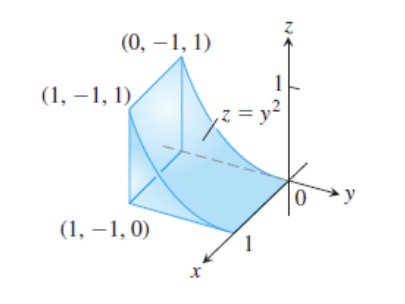
\includegraphics[scale=0.45]{15_5pic.PNG}
	\end{center}
	
	\begin{center}
		(a) $dy \ dz \ dx \quad$
		(b) $dy \ dx \ dz \quad$
		(c) $dx \ dy \ dz \quad$
		(d) $dx \ dz \ dy \quad$
		(e) $dz \ dx \ dy \quad$
	\end{center}
	
	\item Let $D$ be the region bounded by the paraboloid $z=x^2+y^2$ and the 
	plane $z=2y$, i.e. \[D=\{(x,y,z) \in \R^3 \mid x^2+y^2 \leq z \leq 2y\}.\] 
	Write triple iterated integrals in the orders $dz\ dy\ dx$ and  $dx\ dz\ dy$
	that give the volume of $D$.  Can you write a single triple iterated integral for this volume using any other orders of integration?

%%%%%%
\end{enumerate}
}{}

\iftoggle{answers}
{
	\begin{center}{\large \textbf{Math 2551 Worksheet Answers: Triple Integrals}}
	\end{center}

\begin{enumerate}
	\item $\dfrac{-58}{3}$, region of integration the rectangular prism $[-1,1]\times[0,4]\times[0,1]$ or $-1\leq x \leq 1, 0\leq y \leq 4, 0\leq z\leq 1$.

	\item Various possibilities depending on order of integration.  E.g \[\int_0^1 \int_0^{1-x} \int_0^{1-x-y}\ z\ dz\ dy\ dx \]

	\item 
	\begin{enumerate}
		\item $\displaystyle\int_0^1 \int_0^1 \int_{-1}^{-\sqrt z}\ dy \ dz \ dx $
		\item $\displaystyle\int_0^1 \int_0^1 \int_{-1}^{-\sqrt z}\ dy \ dx \ dz  $
		\item $\displaystyle\int_0^1 \int_{-1}^{-\sqrt z} \int_0^1\ dx \ dy  \ dz  $
		\item $\displaystyle\int_{-1}^0 \int_0^{y^2} \int_0^1 \ dx \ dz \ dy$
		\item $\displaystyle\int_{-1}^0  \int_0^1  \int_0^{y^2}\ dz \ dx \ dy$
	\end{enumerate}

	\item $\Ds \int_{-1}^1 \int_{1-\sqrt{1-x^2}}^{1+\sqrt{1-x^2}} \int_{x^2+y^2}^{2y} dz\ dy\ dx$.
	
		$\Ds \int_{0}^{2} \int_{y^2}^{2y} \int_{-\sqrt{z-y^2}}^{\sqrt{z-y^2}} dx\ dz\ dy$.
		
		Yes, all orders of integration result in a single iterated integral.
\end{enumerate}
}{}
\iftoggle{solutions}
{
Solutions go here in the same format.
}{}

 
\fancyhead[C]{Section 15.7}
\fancyhead[R]{\daynineteen}

\section*{\centering Chapter 15.7: Cylindrical and Spherical Coordinates}
\textbf{I3: Change of Variables.} I can use polar, cylindrical, and spherical coordinates to transform double and triple integrals and can sketch regions based on given polar, cylindrical, and spherical iterated integrals. I can use general change of variables to transform double and triple integrals for easier calculation.  I can choose the most appropriate coordinate system to evaluate a specific integral.\\\\
During studio, focus on \textit{setting up} the integrals. However, don't forget to carry out the actual integration in your own time. Both the correct triple integral and correct final answer are given in the answers for this worksheet.
\subsection*{Mechanics}
\begin{enumerate}
    \item \question{
    Use spherical coordinates to verify that the volume of a sphere with radius $\rho$ is $\dfrac{4}{3}\pi \rho^3$.
    }
        {% answer here
        
        }
        {% solution here
        
        }
    	
	\item \question{Use cylindrical coordinates to compute $\displaystyle \int_{-1}^1 \int_0^{\sqrt{1-y^2}} \int_0^x (x^2+y^2) \ dz \ dx \ dy$}
        {% answer here
        
        }
        {% solution here
        
        }
    
    \item \question{Find the volume of the solid that lies within the sphere $x^2+y^2+z^2=4$, above the $xy$-plane, and below the cone $z=\sqrt{x^2+y^2}$.}
        {% answer here
        
        }
        {% solution here
        
        }
     \item \question{Find the volume of the region bounded above by the paraboloid $z=9-x^2-y^2$, below by the $xy$-plane, and lying \emph{outside} the cylinder $x^2+y^2=1$.}
        {% answer here
        
        }
        {% solution here
        
        }
        \item \question{Suppose $a \geq 0$. Find the volume of the region cut from the solid sphere $\rho \leq a$ by the half-planes $\theta=0$ and $\theta= \pi/6$ in the first octant.}
        {% answer here
        
        }
        {% solution here
        
        }
        \item \question{When might you prefer to use cylindrical coordinates over spherical ones? In other words, is there a particular type of symmetry whose presence/absence suggests that cylindrical coordinates may be more useful?}
        {% answer here
        
        }
        {% solution here
        
        }
\end{enumerate}
\subsection*{Applications}
\begin{enumerate}[resume]
	
	\item \question{Let $D$ be the right circular cylinder whose base is the circle $r=2\sin \theta$ in the $xy$-plane and whose top is the plane $z=4-y$. Recall that $r=2 \sin \theta$ describes a circle centered at $(0,1)$ with radius $1$ in the $xy$-plane. Using cylindrical coordinates,
	\begin{enumerate}
		\item find the volume of the region $D$.
		\item find the $\bar{x}$ component of the centroid of the region. \textit{[Hint: Use symmetry.]}
	\end{enumerate}}
        {% answer here
        
        }
        {% solution here
        
        }
    \item \question{A double-scoop ice cream cone can be modeled by the region bound by the three component surfaces 
    \begin{align*}
        \textrm{Cone: }&9x^2+9y^2 -z^2= 0\qquad &&\textrm{for }0\leq z\leq 6 \\
        \textrm{Scoop One: }&x^2+y^2+(z-8)^2=9  \qquad &&\textrm{for }6\leq z\leq 10\\
        \textrm{Scoop Two: }&x^2+y^2+(z-12)^2 = 9\qquad &&\textrm{for }10\leq z
    \end{align*}
    Compute the volume of the entire dessert (including what is inside the cone, presumably more ice cream). \textit{[Hint: Do not compute the volume of the scoops as they are presented. Translate each scoop down so they are centered at the origin.]}
    \begin{center}
		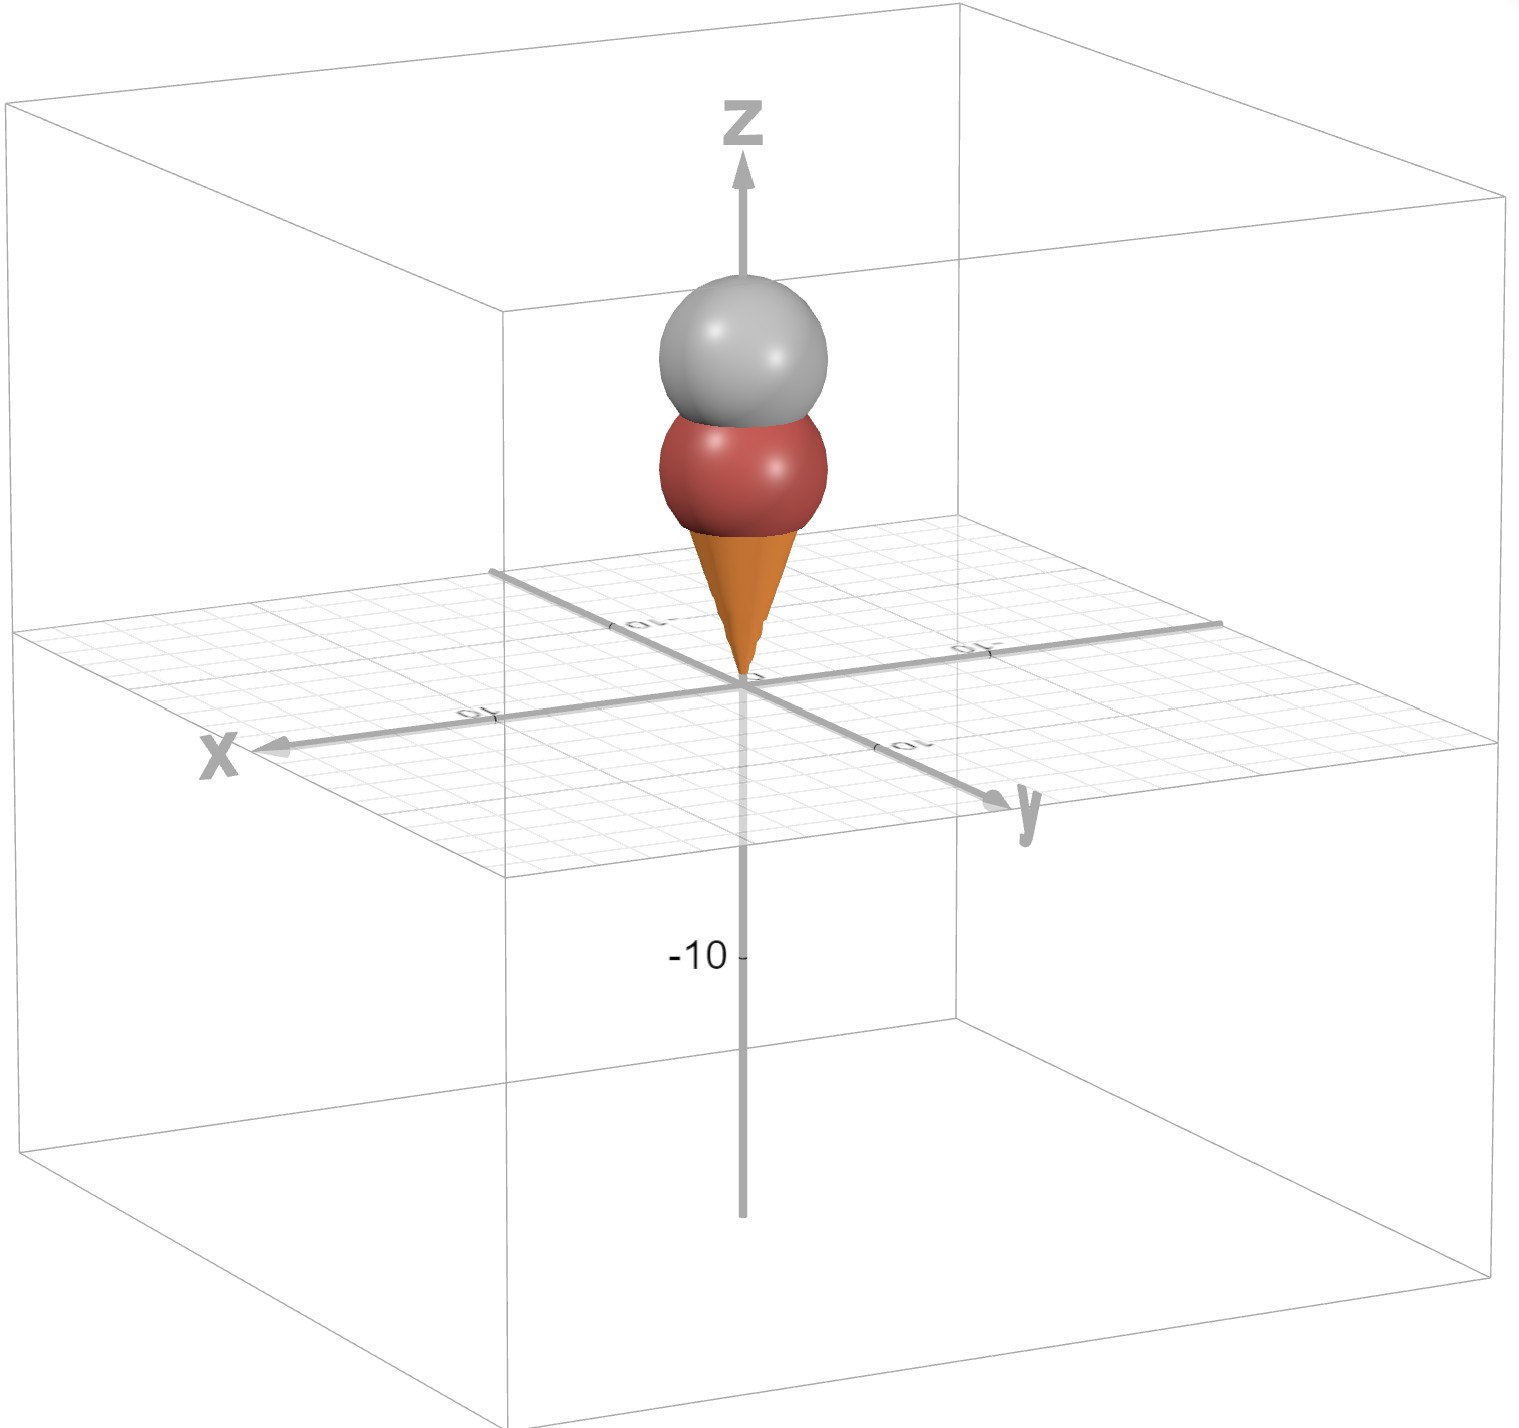
\includegraphics[scale=0.5,alt={ice cream cone and scoops}]{ice creammm.jpg}
	\end{center}}
        {% answer here
        
        }
        {% solution here
        
        }
\end{enumerate}
\subsection*{Extensions}
\begin{enumerate}[resume]
	\item \question{Let $B$ be the unit ball given by $x^2+y^2+z^2\leq 1$. Compute the average distance of a point in $B$ to the origin. Before you do any calculations, do you expect the average to be less than or greater than 0.5? Why? }
        {% answer here
        
        }
        {% solution here
        
        }
	
	\item \question{Find the volume of the solid that is between the spheres $\rho=\sqrt{2}$ and $\rho=2$, but outside of the circular cylinder $x^2+y^2=1$.  It will be helpful to draw a cross-section in a plane $\theta=c$ for this problem and to use symmetry.}
        {% answer here
        
        }
        {% solution here
        
        }

\end{enumerate}
{}

\iftoggle{answers}{
\begin{center}{\large \textbf{Math 2551 Worksheet Answers: Triple Integrals in Cylindrical \& Spherical Coordinates}}
\end{center}

\begin{enumerate}
	\item Integral: $\Ds \int_{-\pi/2}^{\pi/2} \int_0^1 \int_0^{r\cos(\theta)}r^3\ dz\ dr\ d\theta$
	
	Answer: $\dfrac{2}{5}.$
	
	\item Integral: $\Ds \int_0^{\pi/6} \int_0^{\pi/2} \int_0^a \rho^2\sin(\phi)\ d\rho\ d\phi\ d\theta$
	
	Answer: $\dfrac{a^3\pi}{18}.$
	
	\item Integral: $\Ds \int_0^{2\pi} \int_{\pi/4}^{\pi/2} \int_0^2 \rho^2\sin(\phi)\ d\rho\ d\phi\ d\theta$ 
	
	Answer: $\dfrac{8\sqrt{2}\pi}{3}$
	
	\item Integral: $\Ds \int_0^{2\pi} \int_1^3 \int_0^{9-r^2} r\ dz\ dr\ d\theta$
	
	Answer: $32\pi$
	
	\item Integral: $\Ds 2 \left( \int_0^{2\pi}\int_{\pi/6}^{\pi/4} \int_{\csc(\phi)}^{2} \rho^2\sin(\phi)\ d\rho\ d\phi\ d\theta +\int_0^{2\pi}\int_{\pi/4}^{\pi/2} \int_{\sqrt{2}}^{2} \rho^2\sin(\phi)\ d\rho\ d\phi\ d\theta \right)$
	
	Answer: $\dfrac{12\sqrt{3}-4}{3}\pi $.
	
	\item \begin{enumerate}
		\item Integral: $\Ds \int_0^{\pi} \int_0^{2\sin(\theta)} \int_0^{4-r\sin(\theta)} r\ dz\ dr\ d\theta$
		
		Answer: $3\pi.$
		\item $\bar{x}=0$.
	\end{enumerate}
\end{enumerate}

}{}
\iftoggle{solutions}
{
Solutions go here in the same format.
}{}

 \fancyhead[C]{Section 15.8}
	\fancyhead[R]{\daytwenty}
	
\iftoggle{questions}{
\begin{center}{\large \textbf{Math 2551 Worksheet: Change of Variables}}
\end{center}

\begin{enumerate}
	
	\item Find the Jacobian determinant of the transformation $x=e^{-r}\sin(\theta), y=e^r\cos(\theta)$.
	
	\item Find the image of the set $S$ which is the disk given by $u^2+v^2\leq 1$ under the transformation\[\bT(u,v)=\begin{bmatrix} au \\ bv\end{bmatrix}\] for some constants $a,b>0$.
	
	Give an example integration problem for which this result would be helpful.
	
	\item Find equations for a transformation $\bT$ that maps a rectangular region $S$ in the $uv$-plane whose sides are parallel to the $u$- and $v$-axes onto the region $R$ bounded by the hyperbolas $y=1/x, y=3/x$ and the lines $y=x, y=3x$ in the first quadrant.
	
	\item Solve the system \[u=2x-3y, v=-x+y \] for $x$ and $y$ in terms of $u$ and $v$.  Then find the value of the Jacobian and find the image of the parallelogram $R$ in the $xy$-plane with boundaries $x=-3, x=0, y=x,$ and $y=x+1$ under this transformation.  Sketch the transformed region in the $uv$-plane.  Use your results to rewrite the integral \[\iint_R 2(x-y)\ dx\ dy \] as an integral in $uv$-coordinates.
	
	\item Use a change of variables to compute \[ \iint_R xy\ dA, \] where $R$ is the region in the first quadrant bounded by the lines $y=x$ and $y=3x$ and the hyperbolas $xy=1, xy=3$.  
	
	Hint: Think about problem 3 above.	
	
	\item Compute $\Ds \iint_R e^{x+y}\ dA$, where $R$ is the region given by the inequality $|x|+|y|\leq 1$.
\end{enumerate}
}{}

\iftoggle{answers}
{
	\begin{center}{\large \textbf{Math 2551 Worksheet Answers: Change of Variables}}
	\end{center}

	\begin{enumerate}
		\item $\sin^2(\theta)-\cos^2(\theta)=-\cos(2\theta)$
		
		\item The elliptical region $\dfrac{x^2}{a^2}+\dfrac{y^2}{b^2}\leq 1$.\\
		
		Many possible answers: any such should involve an integration problem where the region of integration is an ellipse with major and minor axes parallel to the $x$ and $y$-axes.
		
		\item $x=\sqrt{\dfrac{u}{v}}, y=\sqrt{uv}$ maps $[1,3]\times[1,3]$ onto $R$	
		
		\item  $\displaystyle\int_0^1 \int_{-3v}^{-3v+3} -2v \ du\ dv $
		
		\item $\ln(9)$
		
		\item $e+\dfrac{1}{e}$
	\end{enumerate}
}{}
\iftoggle{solutions}
{
Solutions go here in the same format.
}{}

% \fancyhead[C]{Section 16.1}
	\fancyhead[R]{\daytwentyone}

\iftoggle{questions}{
\begin{center}{\large \textbf{Math 2551 Worksheet: Scalar Line Integrals}}
\end{center}

\begin{enumerate}
	\item For each curve, find a parameterization of the curve with the specified orientation.
	\begin{enumerate}
		\item The line segment in $\R^3$ from $(0,1,-2)$ to $(3,-1,2)$.
		
		\item The line segment in $\R^3$ from $(3,-1,2)$ to $(0,1,-2)$.
		
		\item The circle of radius 3 in $\R^2$ centered at the origin, beginning at the point $(0,-3)$ and proceeding clockwise around the circle.
		
		\item In $\R^2$, the portion of the parabola $y^2=x$ from the point $(4,2)$ to the point $(1,-1)$.\\
	\end{enumerate}
	
	For problems 2 to 4 below, do the set up of each line integral before doing any computations.
	
	\item Find the line integral of $f(x,y,z):=\sqrt{x^2+y^2}$ over the curve 
	$\br(t)= \vecf{(-4\sin t)}{+(4\cos t)}{+3t},$ $t \in [0,2\pi]$.\\
	
	\item Find the line integral of $f(x, y) =\sqrt{4x+1}$ over $C$ where $C$ is the part of the curve $x=y^2$ from the point $(4, -2)$ to $(1, 1)$.\\
	
	
	\item Let $C$ be the curve with parameterization
	\[
	\br(t)=\vecf{(e^t \cos t)}{+(e^t\sin t)}{+e^t},\quad t \in [0,\pi].
	\]
	Find the mass of $C$ if the density of a wire along $C$ is $\delta(x,y,z)=z^{-1}$.\\
	
	
	
	\textbf{Vector Field Problems:} In Chapter 13, we talked about vector-valued functions: functions whose input is a single real number and whose output is a vector in $\R^2$ or $\R^3$.  A very important related type of function in this unit is a \textbf{vector field}, which is a function that takes a point $(x,y)$ in $\R^2$ and outputs a vector in $\R^2$ or a point $(x,y,z)$ in $\R^3$ and outputs a vector in $\R^3$.
	
	\item If we want to make a decision based on what the wind is doing, then we need to keep track of not just its strength at any point, but also its direction! So a vector field is a good model here: at each point $(x,y)$, we can record the velocity vector for the wind.
	
	Suppose that given the point $(x,y)$ in the plane, we know that the wind velocity at that point is given by the vector $\bF(x,y)=\langle y, x\rangle$.  For example, at the point $(1,-1)$, the wind velocity is $\bF(1,-1)=\langle -1,1\rangle$.  Fill in the table below with the wind velocity vectors for the given points.\\
	
	\begin{tabular}{c|c}
		$(x,y)$ & $(-2,0)\quad (-1,2)\quad (0,-2)\quad (1,1)\quad (2,3)\quad (3,2)\quad (-1,0)\quad (1,3)$ \\
		\hline $\bF(x,y)$ &
	\end{tabular}
	
	\pagebreak
	
	\item Another useful way of recording this information is to plot the velocity vectors!  At each point $(x,y)$ we will draw the vector $\bF(x,y)$ starting with the tail of the vector at $(x,y)$.  This has been done for you with the point $(1,-1)$ below.  Fill in the plot with the other vectors you found in the last problem.
	
	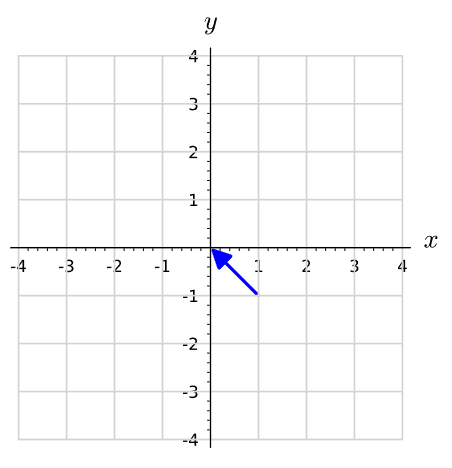
\includegraphics[scale=0.6]{ws_21_plot.png}
	
	CalcPlot3d can graph vector fields too! Use it to check your work and see the full detail of this vector field.
	
	
	\item Let $f(x,y)=\frac{1}{2}(x-y)^2$. Find the gradient vector field, $\nabla f$, of $f$ and sketch it.
\end{enumerate}
}{}

\iftoggle{answers}{
\begin{center}{\large \textbf{Math 2551 Worksheet Answers: Scalar Line Integrals}}
\end{center}
\begin{enumerate}
	\item There are many possible correct answers!  Here are some.
	\begin{enumerate}
		\item $\br(t)=\langle 3t, -2t+1, 4t-2\rangle, \quad 0\leq t \leq 1$
		
		\item  $\br(t)=\langle -3t+3, 2t-1, -4t+2\rangle, \quad 0\leq t \leq 1$
		
		\item $\br(t)=\langle 3 \sin(t), 3\cos(t) \rangle, \quad \pi\leq t\leq 3\pi$
		
		\item $\br(t)=\langle t^2, -t\rangle \quad -2 \leq t \leq 1$
	\end{enumerate}
	\item The integral to compute is $\Ds \int_0^{2\pi} 20\ dt$ since $f(\br(t))=4$ and $\|\br'(t)\|=5$.  Its value is $40 \pi$.
	
	\item The integral to compute is $Ds \int_{-2}^1 4t^2+1\ dt$. Its value is $15$.
	
	
	\item The integral to compute is $Ds \int_0^{\pi} e^{-t}e^t\sqrt{3}\ dt$ $\sqrt{3}\pi$
	
	
	\item	
	\begin{tabular}{c|c}
		$(x,y)$ & $(-2,0)\quad (-1,2)\quad (0,-2)\quad (1,1)\quad (2,3)\quad (3,2)\quad (-1,0)\quad (1,3)$ \\
		\hline $\bF(x,y)$ & $\langle 0, -2 \rangle\quad \langle 2,-1\rangle\quad \langle -2, 0 \rangle \quad \langle 1,1 \rangle \quad \langle 3,2 \rangle \quad \langle 2,3 \rangle \quad \langle 0, -1 \rangle \quad \langle 3, 1\rangle$
	\end{tabular}
	
	\item \begin{minipage}{0.5\textwidth}Without rescaling vectors to fit better:
		
		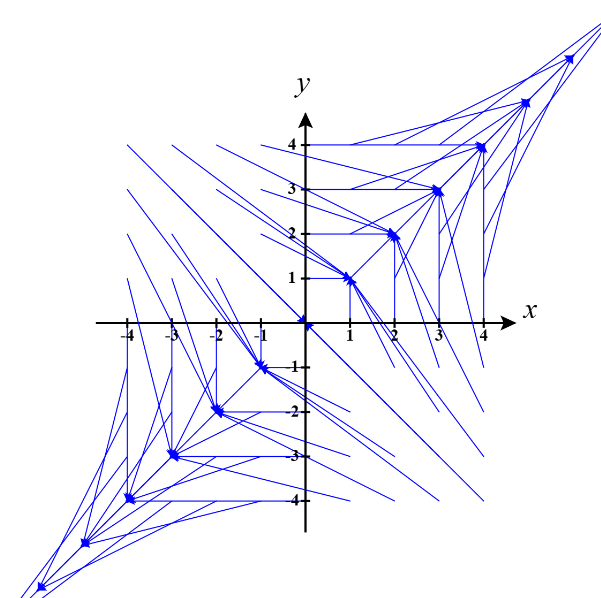
\includegraphics[scale=0.4]{ws_21_plot_ans_noscale.png}
	\end{minipage}\begin{minipage}{0.5\textwidth}
	With rescaling:
	
	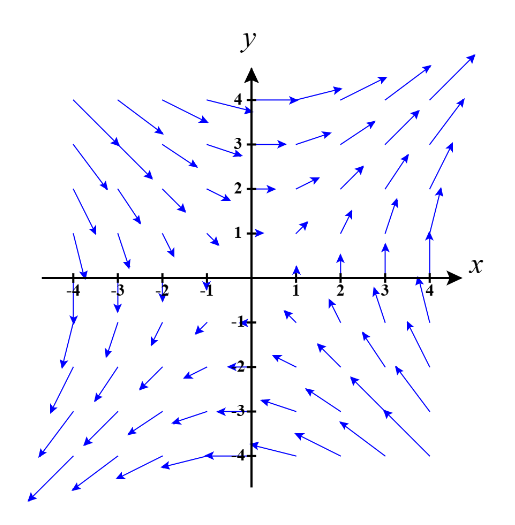
\includegraphics[scale=0.4]{ws_21_plot_ans.png}
\end{minipage}
	
	\item $\nabla f(x,y)=\langle x-y,y-x\rangle$
\end{enumerate}
}{}
\iftoggle{solutions}
{
Solutions go here in the same format.
}{}

% \fancyhead[C]{Section 16.2}
	\fancyhead[R]{\daytwentytwo}

\iftoggle{questions}{
\begin{center}{\large \textbf{Math 2551 Worksheet: Vector Line Integrals}}
\end{center}

\begin{enumerate}
	
	\item Consider the vector field $\bF$ (thin arrows) and and let $\bT$ denote the unit tangent vector to the directed curves shown below (denoted with thick arrows). Determine whether \[ \int_C \bF\cdot\bT\ ds\] is positive, negative, or zero for each directed curve $C$.  In other words, determine whether the \textit{work} done by the vector field on each curve is positive, negative, or zero.
	
	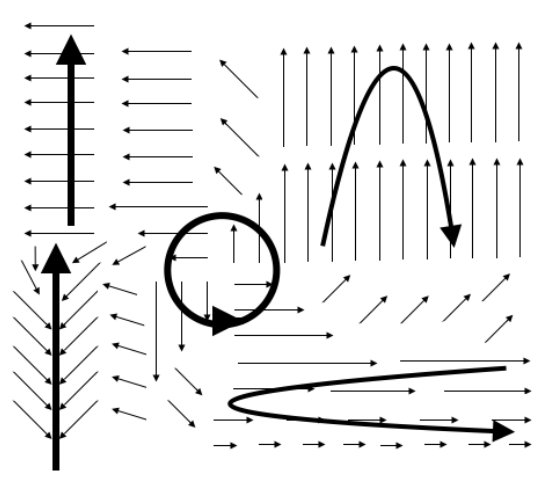
\includegraphics[scale=0.5]{16_2pic.png}
	
	
	\item Evaluate $\int_C (2x -y)\bi\cdot\ d\br$ where $C$ is parameterized by 
	$\br(t) = (t^2)\bi+(3t-2)\bj$ , $t \in [0,1]$.\\
	
	\item Find the work done by the force $\bF= xy \bi +(y-x) \bj$ over the straight line from $(1,1)$ to $(2,3)$.\\
	
	\item Consider the closed curve $C$ consisting of a semicircle and a straight line segment as follow:
	\[
	\br_1(t)=(2 \cos t)\bi+(2 \sin t)\bj, \ t \in [0,\pi], \qquad \br_2(t)=t\bi, \ t\in [-2,2]
	\]
	Let the vector field $\bF$ be given by 
	\[
	\bF(x,y) = -y^2 \bi + x^2 \bj.
	\]
	Find the circulation of $\bF$ around $C$ and the flux of $\bF$ across $C$. 
	%%
	
	\item Give an example of a non-trivial force field $\bF$ (not the zero vector at all points) and a non-trivial path $\br(t)$ (not the stationary path at a point $P$) for which the total work done moving along the path is zero.
\end{enumerate}
}{}

\iftoggle{answers}{
\begin{center}{\large \textbf{Math 2551 Worksheet Answers: Vector Line Integrals}}
\end{center}
\begin{enumerate}
	\item Top left: 0 \\
	Bottom left: Negative \\
	Center: Positive \\
	Top right: 0\\
	Bottom right: Negative
	
	
	\item 1
	
	\item $\dfrac{25}{6}$
	
	\item Circulation: $\dfrac{32}{3}$\\
	Flux: 0
	
	\item Many possible examples: the top left and top right examples from 1), $\nabla f$ for any $f$ together with a closed curve $\br$, any example where $\bF\cdot \br'(t)=0$, i.e. the field and curve are orthogonal, and more.
\end{enumerate}
}{}
\iftoggle{solutions}
{
Solutions go here in the same format.
}{}

% \fancyhead[C]{Section 16.3}
	\fancyhead[R]{\daytwentythree}
	
\iftoggle{questions}{
\begin{center}{\large \textbf{Math 2551 Worksheet: Potentials and Conservative Vector Fields}}
\end{center}

\begin{enumerate}
	\item Show that the vector field $\bF=12xy\bi+6(x^2+y^2)\bj$ is conservative using the mixed partials test, then find a potential function $f$ such that $\bF=\nabla f$.
	
	\item Find a potential function $f$ for 
	\[
	\bF(x,y,z) = \vecf{2xy}{+(x^2-z^2)}{-2yz}.
	\]
	Evaluate 
	\[
	\int_C \bF \dotp d\br
	\]
	where $C$ is any path from $(0,0,0)$ to $(1,2,3)$.
	
	\item Let $a,b,c,d,e$ be real numbers and
	\begin{align*}
		P(x,y,z) &= 3x + 7y + 2z; \\
		Q(x,y,z) &= ax+by+4z; \\
		R(x,y,z) &= cx+dy+ez.
	\end{align*}
	For which values of the constants $a,b,c,d,e$ is $\bF = \vecf{P}{+Q}{+R}$ a conservative vector field?
	
	\item Find a potential function $f$ for \[\bF(x,y,z)=\langle \dfrac{1}{y}, -\dfrac{x}{y^2}, 2z-1\rangle\] and use it to evaluate $\int_C \bF\dotp d\br$ along the curve $C: \br(t)=\langle \sqrt{t}, t+1, t^2\rangle, 0\leq t \leq 1$.
	
	\item Compute $\int_C \bF\cdot d\br$ for the vector field $\bF=\left\langle \dfrac{-y}{x^2+y^2},\dfrac{x}{x^2+y^2}\right\rangle$ where the curve C is the unit circle oriented counterclockwise.

\end{enumerate}}{}

\iftoggle{answers}
{
	\begin{center}{\large \textbf{Math 2551 Worksheet Answers: Potentials and Conservative Vector Fields}}
	\end{center}
	
	\begin{enumerate}
		\item $f(x,y)=12x^2y+2y^3$
		
		\item $f(x,y,z)= x^2y-z^2y$ and $\displaystyle \int_C\bF \cdot d\br =-16$.
		
		\item $7=a, 2=c, 4=d$, no restriction on $b$ or $e$.
		
		
		\item $f(x,y,z)= \dfrac{x}{y}+z^2-z$. \\
		$\int_C \bF\dotp d\br = 1/2$   
		
		\item $2\pi$
	\end{enumerate}
}{}
\iftoggle{solutions}
{
Solutions go here in the same format.
}{}

% \fancyhead[C]{Section 16.4}
	\fancyhead[R]{\daytwentyfour}

\iftoggle{questions}{
\begin{center}{\large \textbf{Math 2551 Worksheet: Curl, Divergence, Green's Theorem}}
\end{center}


\begin{enumerate}
	
	\item Below is a plot of a vector field $\bF(x,y)$.  Use this to decide whether the values of $\curl \bF \cdot \bk$ and $\Div \bF$ in each quadrant are positive, negative, or zero.
	
	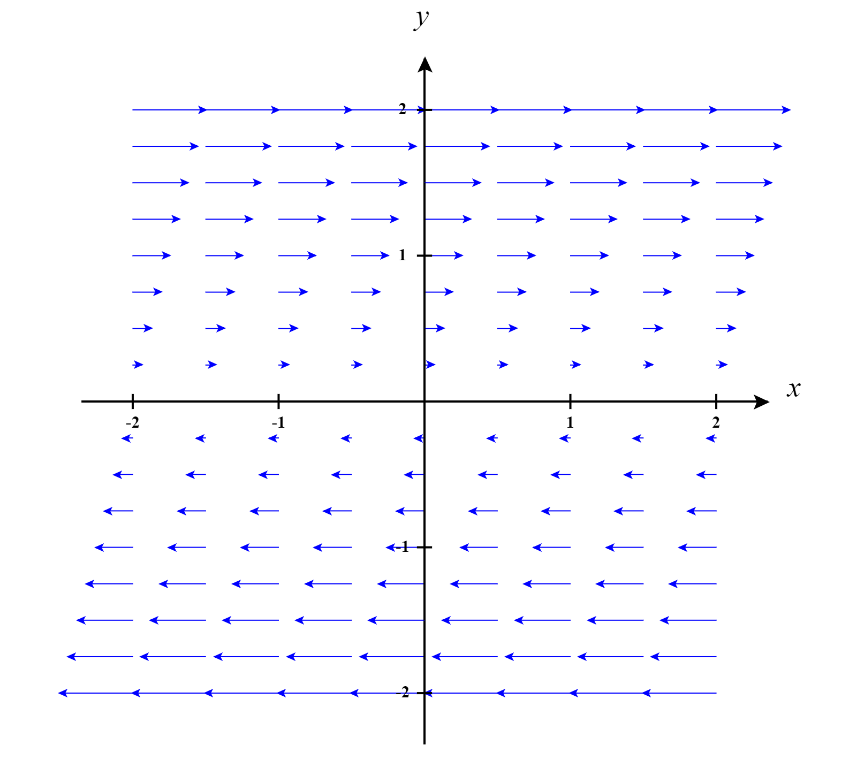
\includegraphics[scale=0.3]{16_3-4pic.png}
	
	\item Compute $\Div \bF$ and $\curl \bF\cdot \bk$ for the vector field $\bF(x,y)=\langle \dfrac{y}{4}, 0 \rangle$, which was plotted above.
	
	%%
	\item Let $C$ be the ellipse 
	\[
	\left( \frac{x}{3} \right)^2 + \left( \frac{y}{4}\right)^2=1.
	\]
	\begin{enumerate}
		\item Parametrize this ellipse to give it a positive orientation.
		
		\item Let $\bF(x,y)=2x \bi + 2y \bj$. Use Green's theorem to find the circulation of $\bF$ around $C$ and its flux across $C$.
	\end{enumerate}  
	\item Let $R$ be the region in the $xy$-plane bounded above by the curve $y=3-x^2$ and below by the curve $y=x^4+1$. Orient this boundary positively. Let 
	\[
	\bF(x,y) = (y+e^x \ln y) \bi + (e^x/y)\bj.
	\]
	Use Green's theorem to find the circulation of $\bF$ around $C$. What happens when you try to use Green's theorem to evaluate the flux of $\bF$ across $C$? Should you use Green's theorem to evaluate the flux integral?
	
	\item Use Green’s Theorem to find the work done by the force $\bF(x,y)=\langle x(x+y),xy^2\rangle$ in moving a particle from the origin along the $x$-axis to $(1,0)$, then along the line segment to $(0,1)$, and then back to the origin along the $y$-axis.
	
	\item \textbf{Looking ahead:} Find a parameterization (a function $\br(s,t)=\langle x(s,t), y(s,t), z(s,t)\rangle$) of the plane through the origin that contains the vectors $\bi-\bj$ and $\bj-\bk$.  Linear algebra ideas may be useful.	
	
\end{enumerate}
}{}

\iftoggle{answers}
{
	\begin{center}{\large \textbf{Math 2551 Worksheet Answers: Curl, Divergence, Green's Theorem}}
	\end{center}

\begin{enumerate}
	
	\item $\nabla\cdot \bF$ is 0 in all quadrants.\\
	$(\nabla \times \bF)\cdot \bk$ is negative in all quadrants.
	
	\item $\nabla\cdot \bF = 0$\\
	$(\nabla \times \bF)\cdot \bk=-\dfrac{1}{4}$. \\
	
	
	\item\begin{enumerate}
		\item $\br(t)=\langle 3 \cos(t), 4\sin(t) \rangle$, $0\leq t \leq 2\pi$.
		
		\item Circulation: 0\\
		Flux: $48\pi$
	\end{enumerate}  
	
	\item Circulation: $-44/15$\\
	Flux: The integrand is very difficult to work with, so we should not use Green's theorem here.
	
	\item $-1/12$
	
	\item One answer (linear algebra!) $\br(s,t)=s\langle 1,-1,0\rangle+t\langle0,1,-1\rangle = \langle s,t-s,-t \rangle$, $s,t\in\R$.
\end{enumerate}
}{}
\iftoggle{solutions}
{
Solutions go here in the same format.
}{}

% \fancyhead[C]{Section 16.5}
	\fancyhead[R]{\daytwentyfive}

\iftoggle{questions}{
\begin{center}{\large \textbf{Math 2551 Worksheet: Surfaces}}
\end{center}


\begin{enumerate}
	
	\item Consider the surface cut from the parabolic cylinder $y=4-x^2$ by the planes $z=0$, $z=2$, and $y=0$. Sketch $S$ and find a parameterization of $S$.
	
	\item Consider the surface left in the hemisphere $x^2+y^2+z^2=4, \ z\geq 0$ after cutting off the lower part between the planes $z=0$ and $z=\sqrt{3}$ from the hemisphere. (In short, $S$ is the surface which is the part of $x^2+y^2+z^2=4$ above $z=\sqrt{3}$). Sketch $S$, parametrize $S$ and find the surface area of $S$. 

	\item The tangent plane at a point $P_0=(f(u_0,v_0),g(u_0,v_0),h(u_0,v_0))$ on a parameterized surface $\br(u,v)=\langle f(u,v), g(u,v) ,h(u,v)\rangle$ is the plane through $P_0$ normal to the vector $\br_u (u_0,v_0)\times\br_v(u_0,v_0)$.\\
	
	Use this to find an equation to the tangent plane of the surface parameterized by $\br(r,\theta)=(r\cos(\theta))\bi+(r\sin(\theta))\bj+r\bk, r\geq 0, 0\leq\theta\leq 2\pi$ at the point where $(r,\theta)=(2,\pi/4)$.\\
	
	What is a Cartesian equation for this surface?  Sketch it and the tangent plane.

	\item Find the area of the part of the surface $z=xy$ that lies within the cylinder $x^2+y^2=1$. \\

	\item Find the area of the surface cut from the ``nose" of the paraboloid $x=1-y^2-z^2$ by the $yz$-plane.\\
\end{enumerate}
}{}

\iftoggle{answers}{
\begin{center}{\large \textbf{Math 2551 Worksheet Answers: Surfaces}}
\end{center}

\begin{enumerate}
	
	\item One answer: $\br(u,v)=\langle u, 4-u^2, v\rangle$, $-2\leq u\leq 2, 0\leq v\leq 2$. 
	
	\item One answer: $\br(\phi,\theta)=\langle 2\sin(\phi)\cos(\theta), 2\sin(\phi)\sin(\theta),2\cos(\phi)\rangle$ with $0\leq \phi \leq \pi/6$ and $0\leq \theta \leq 2\pi$.\\
	SA: $8\pi \left(1-\frac{\sqrt{3}}{2} \right)$
	
	\item The tangent plane is $-\sqrt{2}(x-\sqrt{2})-\sqrt{2}(y-\sqrt{2})+2(z-2)=0$. This is the cone $z=\sqrt{x^2+y^2}$.
	
	\item $\dfrac{2}{3}\pi(2^{3/2}-1)$ 
	
	\item $\dfrac{\pi}{6}(5^{3/2}-1)$
\end{enumerate}

}{}
\iftoggle{solutions}
{
Solutions go here in the same format.
}{}
% \fancyhead[C]{Section 16.6}
	\fancyhead[R]{\daytwentysix}
	
\iftoggle{questions}{
\begin{center}{\large \textbf{Math 2551 Worksheet: Surface Integrals}}
\end{center}

\title{Math 2551 Worksheet: Surface Integrals}

\begin{enumerate}

\item Integrate $f(x,y,z)=yz$ over the part of the sphere $x^2+y^2+z^2=4$ that lies above the cone $z=\sqrt{x^2+y^2}$.\\

\item Find the flux of the field $\bF(x,y,z)=x^2\bi+y^2\bj+z^2\bk$ across the surface $S$ which is the boundary of the solid half-cylinder $0\leq z \leq \sqrt{1-y^2}, 0\leq x \leq 2$, with the outward orientation. \\

\item A fluid has density $870\ kg/m^3$ and flows with velocity $\bv=\langle z, y^2,x^2\rangle$, where $x,y,z$ are measured in meters and the components of $\bv$ in meters per second.  Find the rate of flow outward through the cylinder $x^2+y^2=4, 0\leq z \leq 1$.
\end{enumerate}
}{}

\iftoggle{answers}
{
	\begin{center}{\large \textbf{Math 2551 Worksheet Answers: Surface Integrals}}
	\end{center}
	
	
	\begin{enumerate}
		
		\item 0
		
		\item $\dfrac{10\pi}{3}$
		
		\item 0
		
	\end{enumerate}

}{}
\iftoggle{solutions}
{
Solutions go here in the same format.
}{}

% \fancyhead[C]{Section 16.7}
	\fancyhead[R]{\daytwentysix}
	
\iftoggle{questions}{
\begin{center}{\large \textbf{Math 2551 Worksheet: Stokes' Theorem}}
\end{center}
\title{Math 2551 Worksheet: Stokes' Theorem}

\begin{enumerate}

\item Let $H$ be the hemisphere and $P$ be the portion of a paraboloid shown below. Use Stokes' Theorem to explain why, if $\bF$ is a vector field on $\R^3$ whose components have continuous partial derivatives, we must have \[\iint_H (\nabla \times \bF) \dotp \bn\ d\sigma=\iint_P (\nabla \times \bF) \dotp \bn\ d\sigma .\]

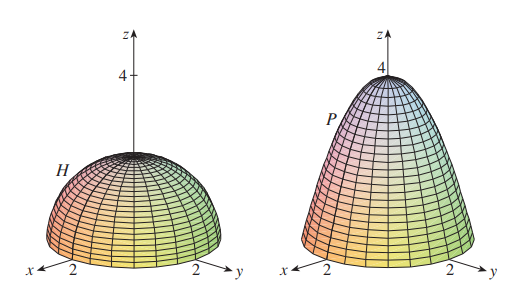
\includegraphics[scale=0.8]{ws_27_ph.png}

\item Use Stokes' Theorem to evaluate $\iint_S (\nabla \times \bF)\dotp \bn\ d\sigma$, where $\bF=\langle x^2z^2,y^2z^2,xyz\rangle$ and $S$ is the part of the paraboloid $z=x^2+y^2$ that lies inside the cylinder $x^2+y^2=4$, oriented upward.

\item A particle moves along line segments from the origin to the points $(1,0,0), (1,2,1),(0,2,1)$, and back to the origin under the influence of the force field
\[\bF(x,y,z)=z^2\bi+2xy\bj+2y^2\bk. \]
Find the work done by the field on the particle.
\end{enumerate}
}{}

\iftoggle{answers}
{
	\begin{center}{\large \textbf{Math 2551 Worksheet Answers: Stokes' Theorem}}
	\end{center}
	
	
	\begin{enumerate}
		
		\item $H$ and $P$ have the same oriented boundary curve $C$ provided that they are oriented in the same way, so by Stokes' theorem the given integrals must be equal.
		
		\item 0
		
		\item 3
	\end{enumerate}

}{}
\iftoggle{solutions}
{
Solutions go here in the same format.
}{}

% \fancyhead[C]{Sections 15.5-15.8, 16.1-16.8}
	\fancyhead[R]{\daytwentyseven}
	
\iftoggle{questions}{
\begin{center}{\large \textbf{Math 2551 Worksheet: Review for Exam 3}}
\end{center}

\title{Math 2551 Worksheet: Review for Exam 3}

\begin{enumerate}
	
	\item Set up an iterated integral in spherical coordinates for $\displaystyle \iiint_E z^2\ dV$ where $E$ is the region between the spheres $x^2+y^2+z^2=4$ and $x^2+y^2+z^2=25$ and inside $z=-\sqrt{\frac{1}{3}(x^2+y^2)}$.
	
	
	\item Set up an integral that computes the volume of the solid which is bounded above by the cylinder $z=4-x^2$, on the sides by the cylinder $x^2+y^2=4$, and below by the $xy$-plane using 
	\begin{enumerate}
		\item Cartesian coordinates
		\item cylindrical coordinates
	\end{enumerate}
	
	Which integral would you rather evaluate and why?

	\item Find an integral that computes the mass of the wire which lies along the curve $y^2=x^3$ from $(0,0)$ to $(1,-1)$ and has density function $\rho(x,y)=2xy^2$.\\

	\item Show that the field $\bF=2x\bi-y^2\bj-\frac{4}{1+z^2}\bk$ is conservative, find a potential function, and use it to compute the integral 
	\[ \int_C 2x\ dx -y^2\ dy - \frac{4}{1+z^2}\ dz \]
	where $C$ is any path from $(0,0,0)$ to $(3,3,1)$.\\
	
	\item Compute $\int_C (6y+x)\ dx + (y+2x)\ dy$ using any method, where $C$ is the circle $(x-2)^2+(y-3)^2=4$.\\

	\item Find the flux of the field $\bF=y\bi-x\bj+\bk$ through the portion of the sphere $x^2+y^2+z^2=a^2$ in the first octant in the direction away from the origin.\\

	\item Use Stokes' theorem to show that the circulation of the field $\bF=\langle 2x, 2y, 2z\rangle$ around the boundary curve $C$ of \textbf{any} smooth orientable surface $S$ in $\R^3$ is 0. \\

	\item Find the outward flux of $\bF = (x\bi+y\bj+z\bk)/\sqrt{x^2+y^2+z^2}$ through the boundary $S$ of the ``thick sphere" $D$ given by the points satisfying $1\leq x^2+y^2+z^2\leq 4$.
\end{enumerate}
}{}

\iftoggle{answers}{
\begin{center}{\large \textbf{Math 2551 Worksheet Answers: Review for Exam 3}}
\end{center}

\begin{enumerate}
	\item $\displaystyle \int_0^{2\pi} \int_{2\pi/3}^\pi\int_2^5 \rho^4 \cos^2(\phi)\sin(\phi) d\rho\ d\phi\ d\theta$ 
	
	
	\item 
	\begin{enumerate}
		\item $\displaystyle \int_{-2}^2 \int_{-\sqrt{4-x^2}}^{\sqrt{4-x^2}} \int_0^{4-x^2}\ dz\ dy\ dx$
		\item $\displaystyle \int_{-2}^2 \int_{-\sqrt{4-x^2}}^{\sqrt{4-x^2}} \int_0^{4-x^2}\ dz\ dy\ dx$
	\end{enumerate}
	
	\item One solution: $\Ds \int_0^1 2(t)(-t^{3/2})^2\sqrt{1+(\frac{3}{2}\sqrt{t})^2}\ dt$.\\
	
	\item $f(x,y,z)=x^2-\frac{1}{3}y^3-4\arctan(z)$.
	
	Integral: $-\pi$. \\
	
	\item $-4\cdot \pi(2)^2$\\
	
	\item $\pi a^2/4$\\
	
	\item $\nabla \times \bF = \langle 0-0,-(0-0),0-0\rangle$ \\
	
	\item $12\pi$
\end{enumerate}

}{}
\iftoggle{solutions}
{
Solutions go here in the same format.
}{}
%\fancyhead[C]{Sections 12.1-6, 13.1-4, 14.1-8, 15.1-8, 16.1-8}
	\fancyhead[R]{\daytwentyeight}
	
\iftoggle{questions}{
\begin{center}{\large \textbf{Math 2551 Worksheet: Review for Final}}
\end{center}

\title{Math 2551 Worksheet: Review for Final}

\begin{enumerate}
	
	\item Find the equation of the plane through $(1,-1,3)$ parallel to the plane $3x+y+z=7$.  Is there a unique plane through $(1,-1,3)$ which is perpendicular to the plane $3x+y+z=7$.  Explain why or why not.
	
	\item Find the point on the curve \[ \br(t)=(5\sin(t))\bi+(5\cos(t))\bj+12t\bk \] at a distance $26\pi$ units along the curve from the point $(0,5,0)$ in the direction of increasing parameter $t$.
		
	\item Find the domain and range of $f(x,y)$ =$\sqrt{x^2-y}$ and identify its level curves.
	
	\item Compute $\displaystyle \lim_{(x,y)\to(0,0)} \frac{y}{x^2-y}$ or show this limit does not exist.
	
	\item Let $f(x,y,z)=xy+2yz-3xz$.  Find the tangent plane to the surface $f(x,y,z)=1$ at $(1,1,0)$ and the linearization $L(x,y,z)$ at $(1,1,0)$.
	
	\item At the point $(1,2)$, the function $f(x,y)$ has a derivative of $2$ in the direction toward $(2,2)$ and a derivative of $-2$ in the direction toward $(1,1)$.  Find $\nabla f(1,2)$ and the derivative of $f$ at $(1,2)$ in the direction toward the point $(4,6)$.	
	
	\item Find the value of the derivative of $f(x,y,z)=xy+yz+xz$ with respect to $t$ on the curve $\br(t)=\langle \cos (t), \sin (t), \cos (2t)\rangle$ at $t=1$.

	\item Find the local minima, local maxima, and saddle points of the function $f(x,y)=x^4-8x^2+3y^2-6y$.

	\item Find the extreme values of $f(x,y)=4xy-x^4-y^4+16$ on the triangular region bounded below by the line $y=-2$, above by the line $y=x$, and on the right by the line $x=2$.

	\item Find the extreme values of $f(x,y)=xy$ on the circle $x^2+y^2=1$.

	\item Sketch the region of integration and reverse the order of integration for the integral
	\[\int_0^{3/2}\int_{-\sqrt{9-4y^2}}^{\sqrt{9-4y^2}}y\ dx\ dy.\]
	
	\item Evaluate the integral \[ \int_{-1}^1\int_{-\sqrt{1-y^2}}^{\sqrt{1-y^2}} \frac{2\ dx\ dy}{(1+x^2+y^2)^2} \] by changing to polar coordinates.
	
	\pagebreak

	\item Find the centroid of the region bounded by the lines $x=2,y=2$, and the hyperbola $xy=2$ in the $xy$-plane.

	\item Find the volume of the region bounded above by the sphere $x^2+y^2+z^2=2$ and below by the paraboloid $z=x^2+y^2$.

	\item Use the transformation $u=3x+2y, v=x+4y$ to evaluate the integral \[\iint_R (3x^2+14xy+8y^2)\ dx\ dy \] where $R$ is the region in the first quadrant bounded by the lines $y=(-3/2)x+1, y=(-3/2)x+3, y=-(1/4)x,$ and $y=-(1/4)x+1)$.
	
	\item Evaluate the integral $\int_C y^2\ dx + x^2\ dy$ where $C$ is the circle $x^2+y^2=4$.
	
	\item Find the outward flux of $\bF=2xy\bi+2yz\bj+2xz\bk$ across the boundary of the cube cut from the first octant by the planes $x=1, y=1, z=1$.

	\item Find the work done by $\bF = \dfrac{x\bi+y\bj}{(x^2+y^2)^{3/2}}$ over the plane curve $\br(t)=\langle e^t \cos(t), e^t\sin(t)\rangle$ from the point $(1,0)$ to the point $(e^{2\pi},0)$.

	\item Find the flux of the field $\bF=\langle 2xy+x, xy-y\rangle$ outward across the boundary of the square bounded by $x=0,x=1,y=0,x=1$.

	\item Find the flux of $\bF = xz\bi+yz\bj+\bk$ across the upper cap cut from the sphere $x^2+y^2+z^2=25$ by the plane $z=3$, oriented away from the $xy$-plane.
\end{enumerate}
}{}

\iftoggle{answers}{
\begin{center}{\large \textbf{Math 2551 Worksheet Answers: Review for Final}}
\end{center}

\begin{enumerate}
	\item $3x+y+z=5$.  There is not a unique plane  because there is not a unique normal direction perpendicular to $\langle 3,1,1\rangle$.
	
	\item $(0,5,24\pi)$
	
	\item Domain $\{(x,y)\mid y\leq x^2\}$
	Range $[0,\infty)$
	Level curves are the parabolas $y=x^2-c^2$ for all $c\geq 0$.
	
	\item The limit does not exist
	
	\item Tangent plane: $(x-1)+(y-1)-z=0$
	Linearization: $L(x,y,z)=1+(x-1)+(y-1)-z$
	
	\item $\nabla f(1,2)=\langle 2,2 \rangle$, $Df_{\bu}(1,2)=14/5$
	
	\item $-\sin^2(1)-\sin(1)\cos(1)+\cos^2(1)+\cos(1)\cos(2)-2\cos(1)\sin(2)-2\sin(1)\sin(2)$
	
	\item $(0,1)$ saddle point, $(2,1), (-2,1)$ local minimum
	
	\item min: -32 at $(2,-2)$  max: 18 at $(1,1)$
	
	\item min: -1/2 at $(1/\pm\sqrt{2},1/\pm\sqrt{2})$ and max: 1/2 at $(1/\pm\sqrt{2},1/\mp\sqrt{2})$.
	
	\item $\Ds \int_{-3}^3 \int_0^{\sqrt{9/4-x^2/4}} y\ dy\ dx$
	
	\item $\pi$
	
	\item $(\bar{x},\bar{y})=\left(\dfrac{1}{2-\ln(4)},\dfrac{1}{2-\ln(4)}\right)$
	
	\item $V=\dfrac{\pi}{6}(8\sqrt{2}-7)$
	
	\item $\dfrac{64}{5}$
	
	\item $0$
	
	\item $3$
	
	\item $1-e^{-2\pi}$
	
	\item $\dfrac{3}{2}$
	
	\item $\dfrac{208\pi}{5}$
\end{enumerate}

}{}
\iftoggle{solutions}
{
Solutions go here in the same format.
}{}

%\fancyhead[C]{Sections 14.3-14.8, 15.1-15.4}
	\fancyhead[R]{HP Review Session}

\iftoggle{questions}{
\begin{center}{\large \textbf{Math 2551 HP Exam 2 Review}}
\end{center}


\begin{enumerate}
	
	
	\item Choose whether each statement is true or false. If the statement is 
	\textit{always} true, pick true. If the statement is \textit{ever} false, 
	pick false.  Give a reason for your answer.
		\begin{enumerate}
			\item If $f_x=f_y$ everywhere, then $f(x,y)$ is constant.
			
			\item There exists a function $f(x,y)$ with $f_x=2x+y$ and 
			$f_y=2x+2y$.
			
			\item If the temperature at a point $(x,y)$ on the floor of a room 
			is given by $T(x,y)$ and heat is being radiated out from a hot spot 
			at the origin, then if $a,b>0$ $\nabla T(a,b)$ could be $\langle 
			2,-2\rangle$.
			
			\item The integral $\iint_R y\ dA$ over the region $R: -1\leq x 
			\leq 1, 0\leq y \leq 1$ is zero.
		\end{enumerate}
	
	\item Based on the contour plot below, determine the signs of the requested 
	derivatives and draw the requested gradients.
	
	\begin{minipage}{0.45\textwidth}
		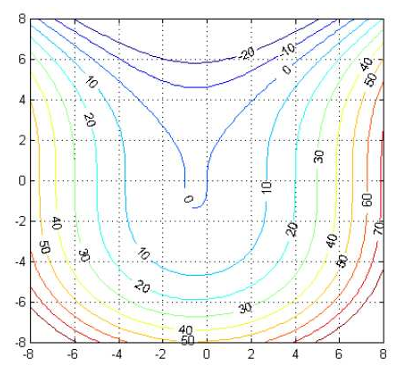
\includegraphics[scale=0.7]{hp_review_contour.png}
	\end{minipage}\begin{minipage}{0.45\textwidth}
	\begin{enumerate}
		\item $f_x(0,0)$ and $f_y(0,0)$
		\item $Df_{\bu}(2,-6)$, $u=\langle1/\sqrt{2},-1/\sqrt{2}\rangle$
		\item $\nabla f(-4,-4)$
		\item The rate of change of $f$ at $(-4,5)$ in the direction towards 
		$(4,6)$
	\end{enumerate}
	\end{minipage}
	
	\item Use the Chain Rule to find the total derivative of the composite 
	function $h=g\circ f$ at the point $(s,t)=(1,1)$, where \[ 
	f(s,t)=\begin{bmatrix}
		s^2+2t \\ 2s-t
	\end{bmatrix}\qquad g(x,y)=3x^2+4y^2.\]
	
	\item Which of the following gaurantees a saddle point of a continuously 
	differentiable function $f(x,y)$ at $(a,b)$?
	\begin{enumerate}
		\item $f_{xx}$ and $f_{yy}$ have the same sign at $(a,b)$
		\item $f_{xx}$ and $f_{yy}$ have opposite signs at $(a,b)$
		\item $f_{xy}$ is negative at $(a,b)$
		\item None of the above.
	\end{enumerate}
	
	\item Find and classify the critical points of $xy-2x-2y-x^2-y^2$. 
	
	\item Find the extreme values of $f(x,y,z)=2x+2y+z$ subject to the 
	constraint $x^2+y^2+z^2=9$. Interpret your results geometrically.
	
	\item Sketch the region of integration, set up iterated integrals for both 
	orders of integration, then evaluate using the easier order and explain why 
	it is easier. \[\iint_R y^2 e^{xy}\ dA, \quad R: x\geq 0, x\leq y \leq 4.\]
\end{enumerate}
}{}

\iftoggle{answers}{
\begin{center}{\large \textbf{Math 2551 HP Exam 2 Review Answers}}
\end{center}

\begin{enumerate}
	
	\item All are true except b).
	
	
	\item -1
	
	\item $\pm 1$
	
	\item Saddle at $(0,0)$ with $f(0,0)=0$, local min at $(0,2)$ of $-4$, local max at $(-2,0)$ of 4, saddle at $(-2,2)$ with $f(-2,2)=0$
	
	\item $(-1/2, 1/2, 1/2)$ and $(0,1,0)$
		
	\item $\sin(4)$
	
	\item No, this is less than $f(x,y)$ at all points, so it cannot possibly be the average value.
	
	\item $1800\pi$ cubic feet
\end{enumerate}
}{}
\iftoggle{solutions}
{
Solutions go here in the same format.
}{}

%\fancyhead[C]{Sections 15.5-8, 16.1-8}
	\fancyhead[R]{HP Review Session}

\iftoggle{questions}{
\begin{center}{\large \textbf{Math 2551 HP Exam 3 Review}}
\end{center}


\begin{enumerate}
	\item Set up integrals for the volume of the solid $S$ bounded by the three coordinate planes, bounded above by the plane $x+y+z=2$, and bounded below by the plane $z=x+y$ using two different orders of integration.
	
	\item Set up integrals that compute the volumes of the solids:
	\begin{enumerate}
		\item Bounded by $z=x^2+y^2$ and $z^2=4(x^2+y^2)$
		\item Bounded above by the hemisphere $x^2+y^2+z^2=1, z\geq 0$ and below by the \textit{cardioid of revolution} $\rho=1+\cos(\varphi)$
	\end{enumerate}
	
	\item Use change of variables with $u=(x+y)/2, v=(x-y)/2$ to compute \[\iint_R \sin(\frac{x+y}{2})\cos(\frac{x-y}{2})\ dA,\] where $R$ is the triangle with vertices $(0,0), (2,0),$ and $(1,1)$.
	
	\item Use an appropriate method to compute each of the following:
	\begin{enumerate}
			
		\item The flux of the field $\bF(x,y,z)=\langle x,2y,3z\rangle$ through the portion of the plane $x+y/2+z/3=0$ in the first octant oriented away from the origin.
		\item The work done by $\bF(x,y)=x\bi-y\bj$ on a particle moving from $(-1,2)$ to $(1,2)$ along $y=x^2+1$.
		\item The circulation of the field $\bF(x,y)=y\bi-x\bj$ around a circle of radius $4$ about the origin, oriented clockwise.
		\item The flux of the field $\bF(x,y)=x\bi-y\bj$ across the portion of the curve $y=x^2+1$ from $(-1,2)$ to $(1,2)$ with normal vector upward.
		\item The work done by $\bF(x,y)=xy^2\bi+yx^2\bj$ on a particle moving from $(-1,2)$ to $(1,2)$ along $y=x^2+1$.
		\item The circulation of the field $\bF(x,y)=\langle -2z, 3x, -y\rangle$ around the boundary of surface which is the portion of the plane $x+y/2+z/3=0$ in the first octant oriented from $(1,0,0)$ to $(0,2,0)$ to $(0,0,3)$.
		\item The flux of the field $\bF(x,y,z)=\langle x^3,y^3,z^3\rangle$ out of the sphere $x^2+y^2+z^2=1$.
		\item The surface area of the part of the cylinder $x^2+y^2=$ below the plane $x+2y+z=6$ and above the $xy$-plane (there are at least two methods for this).
	\end{enumerate}
		
\end{enumerate}
}{}

\iftoggle{answers}{
\begin{center}{\large \textbf{Math 2551 HP Exam 3 Review Answers}}
\end{center}

\begin{enumerate}
	
	\item 
\end{enumerate}
}{}
\iftoggle{solutions}
{
Solutions go here in the same format.
}{}



\end{document}

\item \textbf{G1: Lines and Planes.} I can describe lines using the vector equation of a line. I can describe planes using the general equation of a plane. I can find the equations of planes using a point and a normal vector. I can find the intersections of lines and planes.  I can describe the relationships of lines and planes to each other. I can solve problems with lines and planes.
		
		\item \textbf{G2: Calculus of Curves.} I can compute tangent vectors to parametric curves and their velocity, speed, and acceleration. I can find equations of tangent lines to parametric curves. I can solve initial value problems for motion on parametric curves.
		
		\item \textbf{G3: Geometry of Curves.} I can compute the arc length of a curve in two or three dimensions and apply arc length to solve problems. I can compute normal vectors and curvature for curves in two and three dimensions.  I can interpret these objects geometrically and in applications.
		
		\item \textbf{G4: Surfaces.} I can identify standard quadric surfaces including: spheres, ellipsoids, elliptic paraboloids, hyperboloids, cones, and hyperbolic paraboloids. I can match graphs of functions of two variables to their equations and contour plots and determine their domains and ranges.

		\item \textbf{G5: Parameterization.} I can find parametric equations for common curves, such as line segments, graphs of functions of one variable, circles, and ellipses.  I can match given parametric equations to Cartesian equations and graphs. I can parameterize common surfaces, such as planes, quadric surfaces, and functions of two variables.

        \item \textbf{D1: Limits of Functions.} I can calculate the limits of some functions of two variables or and apply the Two-Path Test to determine if they do not exist. I can state the definition of continuity for functions of multiple variables.
        
		\item \textbf{D2: Computing Derivatives.} I can compute partial derivatives, total derivatives, directional derivatives, and gradients. I can use the Chain Rule for multivariable functions to compute derivatives of composite functions.
		
		\item \textbf{D3: Tangent Planes and Linear Approximations.} I can find equations for tangent planes to surfaces and linear approximations of functions at a given point and apply these to solve problems.
		
		\item \textbf{D4: Optimization.} I can locate and classify critical points of functions of two variables. I can find absolute maxima and minima on closed bounded sets. I can use the method of Lagrange multipliers to maximize and minimize functions of two or three variables subject to constraints. I can interpret the results of my calculations to solve problems.
		
		\item \textbf{I1: Double \& Triple Integrals.} I can set up double and triple integrals as iterated integrals over any region. I can sketch regions based on a given iterated integral.  
		
		\item \textbf{I2: Iterated Integrals.} I can compute iterated integrals of two and three variable functions, including applying Fubini's Theorem to change the order of integration of an iterated integral.
		
		\item \textbf{I3: Change of Variables.} I can use polar, cylindrical, and spherical coordinates to transform double and triple integrals and can sketch regions based on given polar, cylindrical, and spherical iterated integrals. I can use general change of variables to transform double and triple integrals for easier calculation.  I can choose the most appropriate coordinate system to evaluate a specific integral.
		
		\item \textbf{A1: Interpreting Derivatives.} I can interpret the meaning of a partial derivative, a gradient, or a directional derivative of a function at a given point in a specified direction, including in the context of a graph or a contour plot.
		
		\item \textbf{A2: Integral Applications.}  I can use multiple integrals to solve physical problems, such as finding area, average value, volume, or the mass or center of mass of a lamina or solid. I can interpret mass, center of mass, work, flow, circulation, flux, and surface area in terms of line and/or surface integrals, as appropriate.
		
		\item \textbf{V1: Line Integrals.} I can set up and evaluate scalar and vector field line integrals in two and three dimensions.
					
		\item \textbf{V2: Conservative Vector Fields.} I can test for conservative vector fields and find potential functions. I can state and apply the Fundamental Theorem of Line Integrals.
					
		\item \textbf{V3: Generalizations of the FTC.} I can state and apply Green's Theorem, Stokes' Theorem and the Divergence Theorem to solve problems in two and three dimensions. I can choose which theorem is appropriate for different integrals. I can compute curl and divergence of vector fields.
					
		\item \textbf{V4: Surface Integrals.} I can set up and compute surface integrals for scalar and vector valued functions.